
%%%%%%%%%%%%%%%%%%%%%%% file typeinst.tex %%%%%%%%%%%%%%%%%%%%%%%%%
%
% This is the LaTeX source for the instructions to authors using
% the LaTeX document class 'llncs.cls' for contributions to
% the Lecture Notes in Computer Sciences series.
% http://www.springer.com/lncs       Springer Heidelberg 2006/05/04
%
% It may be used as a template for your own input - copy it
% to a new file with a new name and use it as the basis
% for your article.
%
% NB: the document class 'llncs' has its own and detailed documentation, see
% ftp://ftp.springer.de/data/pubftp/pub/tex/latex/llncs/latex2e/llncsdoc.pdf
%
%%%%%%%%%%%%%%%%%%%%%%%%%%%%%%%%%%%%%%%%%%%%%%%%%%%%%%%%%%%%%%%%%%%


\documentclass[runningheads,a4paper]{llncs}

\usepackage{amssymb}
\setcounter{tocdepth}{3}
\usepackage{graphicx}
\usepackage{times,amsmath,epsfig}
\usepackage[linesnumbered,ruled,vlined]{algorithm2e}
\usepackage{subfigure}

\usepackage{url}
%\urldef{\mailsa}\path|{alfred.hofmann, ursula.barth, ingrid.haas, frank.holzwarth,|
%\urldef{\mailsb}\path|anna.kramer, leonie.kunz, christine.reiss, nicole.sator,|
%\urldef{\mailsc}\path|erika.siebert-cole, peter.strasser, lncs}@springer.com|
%\newcommand{\keywords}[1]{\par\addvspace\baselineskip
%\noindent\keywordname\enspace\ignorespaces#1}


\begin{document}

\mainmatter  % start of an individual contribution

\pagestyle{empty}

% first the title is needed
\title{Efficient Sampling Methods for Shortest Path Query over Uncertain Graphs}

% a short form should be given in case it is too long for the running head
%\titlerunning{Lecture Notes in Computer Science: Authors' Instructions}

% the name(s) of the author(s) follow(s) next
%
% NB: Chinese authors should write their first names(s) in front of
% their surnames. This ensures that the names appear correctly in
% the running heads and the author index.
%
\author{Yurong Cheng
%\thanks{Please note that the LNCS Editorial assumes that all authors have used
%the western naming convention, with given names preceding surnames. This determines
%the structure of the names in the running heads and the author index.}%
\and Ye Yuan \and Guoren Wang \and Baiyou Qiao \and Zhiqiong Wang
}

%
%\authorrunning{Lecture Notes in Computer Science: Authors' Instructions}
% (feature abused for this document to repeat the title also on left hand pages)

% the affiliations are given next; don't give your e-mail address
% unless you accept that it will be published

\institute{College of Information Science and Engineering, Northeastern University, China\\
\email{cyrneu@gmail.com}
}


%
% NB: a more complex sample for affiliations and the mapping to the
% corresponding authors can be found in the file "llncs.dem"
% (search for the string "\mainmatter" where a contribution starts).
% "llncs.dem" accompanies the document class "llncs.cls".
%

%\toctitle{Lecture Notes in Computer Science}
%\tocauthor{Authors' Instructions}
\maketitle


\begin{abstract}

Graph has become a widely used structure to model data. Unfortunately, data are inherently with uncertainty because of the occurrence of noise and incompleteness in data collection. This is why uncertain graphs catch much attention of researchers. However, the uncertain graph models in existing works assume all edges in a graph are independent of each other, which dose not really make sense in real applications. Thus, we propose a new model for uncertain graphs considering the correlation among edges sharing the same vertex. Moreover, in this paper, we mainly solve the shortest path query, which is a funduemental but important query on graphs, using our new model. As the problem of calculating shortest path probability over correlated uncertain graphs is \#P-hard, we propose different kinds of sampling methods to efficiently compute an approximate answer. The error is very small in our algorithm, which is proved and further verified in our experiments.

%\keywords{Correlated Uncertain Graphs, Shortest Path, Sampling}
\end{abstract}


\section{Introduction}
\label{sec:intro}

\vspace{-0.3cm}

In recent decades, graph has emerged to be a popular structure to model data in database community. The road network data, social network data, biological network data, RDF data, etc., are well-known graph data. However, these data are usually uncertain because noise and incompleteness inevitably exist when collecting data in real applications. For example, researchers usually use sensors in road networks to test all kinds of data such as vehicle speed. Due to the limitation of hardware, sensors may delay or miss some data messages, which causes some inaccuracy to the collected data. Given another example, in the \emph{Protein-Protein Interaction (PPI)} network, the proteins obtained from experiments may either contain some nonexisting protein interactions, or miss some existing ones. So this is the reason why uncertain graphs catch a lot of researches' attentions in recent years~\cite{adar2007managing}\cite{asthana2004predicting}\cite{lian2011efficient}\cite{nierman2002protdb}.

As a fundamental and important query on graphs, shortest path query has a wide application. Taking an example, when a tourist arrives in a new city, he would like to know how to get to a place of interest from his current location using the least time. Though the shortest path query has been studied for a long time, there are few works that cope with it over uncertain graphs.

The existing ones consider the edges of an uncertain graph are independent of each other~\cite{yuan2010efficiently}\cite{zou2011top}. Specifically, given an uncertain graph $\mathcal{G}(V,E,W,Pr)$, its vertices are deterministic, and each edge $e\in E$ is labeled by a two-tuple pair $(w,pr)$, where $w\in W$ is the weight of the edge and $pr\in Pr$ is the existence probability of the edge. A \emph{possible world graph} $g$ is an instance of $\mathcal{G}$. The probability of a \emph{possible world graph} equals to,

\vspace{-0.2cm}
\[
\small{
Pr(g)=
\prod_{\small{e\in E_i}}
pr_i
\prod_{\small{e\not\in E_i}}
(1-pr_i)
}
\]

The shortest path probability $SPr$ of a path is the sum of the probability of all the \emph{possible world graphs} in which it is shortest between the query points. The follows is an example of calculating the shortest path probability under the independent uncertain graph model.

\begin{example}

\vspace{-1cm}
\begin{figure}[htbp]
\centering
  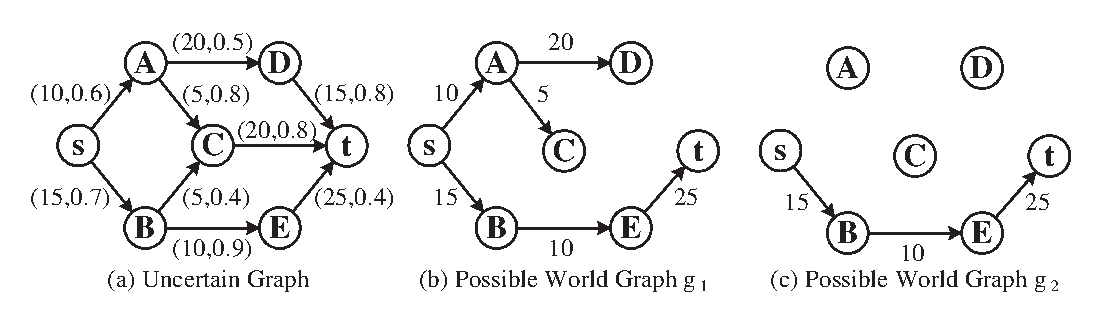
\includegraphics[width=0.99\textwidth]{fig-indep-ug.eps}
\vspace{-0.5cm}
  \caption{\small{Independent Uncertain Graph Model}}
  \label{fig:indep-ug}
\vspace{-0.7cm}
\end{figure}

Fig.~\ref{fig:indep-ug}(a) shows an uncertain graph $\mathcal{G}$ under the independent uncertain graph model, and Fig.~\ref{fig:indep-ug}(b)-(c) are two \emph{possible world graphs} of $\mathcal{G}$, $g_1$ and $g_2$ respectively. The probability of $g_1$ equals to
\vspace{-0.2cm}
\[
Pr(g_1)=0.6\times0.7\times0.5\times0.8\times(1-0.8)\times(1-0.4)\times0.9\times(1-0.8)\times0.4=0.00145
\vspace{-0.2cm}
\]
Among all the \emph{possible world graphs}, there are some ones in which the path $P_{sBEt}$ is the shortest path, such as $g_1$, $g_2$, etc. Thus, the shortest path probability of $P_{sBEt}$ is $SPr(P_{sBEt})=Pr(g_1)+Pr(g_2)+\cdots$
\vspace{-0.2cm}
\end{example}

However, in real applications, the edges are usually not independent of each other. In other words, there are always some hidden correlationships among the edges sharing the same vertex. For example, assuming Fig.~\ref{fig:indep-ug}(a) represents a road network, if a car is known to travel fluently on one road $e_{sB}$, it will be more possible to still travel fluently after it goes across an intersection $B$ to another road $e_{BE}$. Therefore, whether the car travels fluently on edge $BE$, to some extent, depends on whether it travels fluently on edge $sB$. However, the independent model cannot present such correlation among edges such as $BE$ and $sB$. So the independent uncertain graph model is not good enough to describe the real life uncertain graphs.

\textbf{Is there a more reasonable model to describe the uncertain graphs?} In this paper, we propose a new uncertain graph model. This new model can show the correlationship among the edges sharing the same vertex, which overcomes the shortcoming of the existing uncertain graph model.

\textbf{How can we get the query answers efficiently and effectively?} It can be seen that calculating the shortest path probability over correlated uncertain graph is a \#P-hard problem (in Section~\ref{sec:sec:pro-state}). A naive method is to find out all the \emph{possible world graphs}, compute the shortest path in each \emph{possible world graph}, and sum up the corresponding probabilities of the \emph{possible world graphs} whose shortest path is the same. This method is apparently infeasible since the number of \emph{possible world graphs} is exponential, which is impossible to be enumerated.

Thus, in this paper, we first propose a baseline sampling algorithm based on \emph{Monte Carlo} theory, and then design an improved sampling algorithm based on \emph{Unequal Probability Sampling}. The improved algorithm has a less processing time and can provide a more accurate result.

\vspace{-0.5cm}
\subsubsection*{Summery of our contributions and organization:}

\begin{itemize}
\vspace{-0.2cm}
\item	We propose a new Uncertain Graph Model for the shortest path query.
\item   We propose a more effective and efficient sampling algorithm for shortest path query under our model.
\item   We conduct a comprehensive experiment and verify that our improved algorithm can answer the shortest path query more efficiently and accurately than the baseline algorithm.
\vspace{-0.2cm}
\end{itemize}

In the rest of our paper, we introduce our new model and define the problem formally in Section~\ref{sec:model-ProState}. In Section~\ref{sec:base}, we introduce the baseline sampling algorithm. In Section~\ref{sec:impro-samp}, we describe our improved sampling method. In Section~\ref{sec:exp}, we report our experiment results. Finally, we briefly review the related works in Section~\ref{sec:relate} and make a conclusion in Section~\ref{sec:conclu}. Some frequently used symbols in this paper are listed in Table~\ref{tab:note}.

\begin{table}[htbp]
\vspace{-0.5cm}
  \centering
  \caption{\small{Main Symbols}}
\vspace{-0.2cm}
  \label{tab:note}
\scalebox{1}{
  \begin{tabular}{|c|c|c|c|}
    \hline
    \bfseries {Symbols} & \bfseries {Description} & \bfseries {Symbols} & \bfseries {Description}\\
    \hline
    \emph{DAG} & \emph{Directed Acyclic Graph} & $\mathcal{G}$ & uncertain graph\\
    \hline
    $g_c$ & deterministic graph ignoring uncertainty  & $P$ & path\\
    \hline
    \emph{pmf} & \emph{probability mass function} & $SPr$ & shortest path probability \\
    \hline
    \emph{CPr} & conditional probability & \emph{CPT} & Conditional Probability Table \\
    \hline
    $s$ & the source query vertex & $t$ & the terminal query vertex\\
    \hline
    $e_s$ & the edge outgoing $s$ & $v_z$ & a vertex whose in-degree is zero \\
    \hline
    $s_z$ & a source vertex whose in-degree is zero & \emph{MSE} & \emph{Mean Square Error}\\
    \hline
  \end{tabular}
  }
\vspace{-1cm}
\end{table}


\section{The New Uncertain Graph Model and Problem Statement}
\label{sec:model-ProState}

\vspace{-0.3cm}
In this paper, we use directed graphs due to the wide applications in real life. For example, in a road network, it is common to see vehicles stuck in one direction, while the opposite direction has a very light traffic. What's more, in other domains, such as semantic Web (RDF), social networks, and bioinformations, graphs are often directed. Specifically, we take \emph{DAG(Directed Acyclic Graph)} typically in our model, since the cyclic graphs can equivalently be changed into \emph{DAG}s by merging the strong connected components into a single vertices~\cite{zhang2013efficient}. We give the definition of \emph{DAG} as follows.

\vspace{-0.3cm}
\begin{definition}[Directed Acyclic Graph (DAG)]
\label{def:DAG}
A Directed Acyclic Graph is denoted as $DAG(V,E,W)$, where $V$ is the vertex set, $E$ is the edge set, and each edge is given a weight $w\in W$. For any path $P$ from $v_1$ to $v_2$ in a $DAG$, there should be no such paths $P'$s from $v_2$ to $v_1$. If there is an edge $e(v_1,v_2)\in E$, it is called \textbf{outgoing} $v_1$ and \textbf{injecting} $v_2$, and $v_1$ is called a \textbf{parent vertex} of $v_2$. If there are two edges $e_1(v_1,v_2)$ and $e_2(v_2,v_3)$, $e_1$ is called a \textbf{parent edge} of $e_2$. The total number of edges outgoing a vertex is called the \textbf{out-degree} of this vertex, and the total number of edges injecting a vertex is called its \textbf{in-degree}. The vertices with zero in-degree are called \textbf{root vertices}.
\end{definition}
\vspace{-0.3cm}

In this section, we first describe our new uncertain graph model in Section~\ref{sec:sec:model}. Then, in Section~\ref{sec:sec:pro-state}, we formally define our problem.

\vspace{-0.3cm}
\subsection{Uncertain Graph Model}
\label{sec:sec:model}

\vspace{-0.1cm}
\begin{definition}[Uncertain Graph Model]
  \label{def:ug}
  An Uncertain Graph is denoted as $\mathcal{G}(g_c,Pr)$, where $g_c(V,E,W)$ is a \emph{DAG} and $Pr$ is a \emph{probability mass function (pmf)} showing the correlation among edges and their parent edges. Similar to \emph{Bayesian Network}, the \emph{pmf} is represented by a conditional probability $CPr_{e}$ that edge $e$ exists (or not) on the condition that its parent edges exist (or not). That is,
\vspace{-0.3cm}
{\setlength\arraycolsep{2pt}
\begin{eqnarray}
\small
\label{eq:CPrmeaning}
\ CPr_{state(e)} & = & Pr(state(e) | state(e_1),\dots, state(e_i), \dots, state(e_{in}))
\vspace{-0.6cm}
\end{eqnarray}
}
where $e_1$ \dots $e_{in}$ are the parent edges of $e$, and $state(e)$ is the function presenting whether $e$ exists. If $e$ exists, $state(e)=1$. Otherwise, $state(e)=0$.

A conditional probability table \emph{CPT} is used on $e$ to list all its $CPr$s.
\vspace{-0.2cm}
\end{definition}

\vspace{-0.2cm}
\begin{example}[Uncertain Graph Model]
\label{eg:model}
Fig.~\ref{fig:CPT} shows an uncertain graph, and Gi.~\ref{fig:CPT}(a) is its $g_c$. As there are 9 edges in $g_c$, there should be 9 \emph{CPT}s in total, and Fig.~\ref{fig:CPT}(b)-(f) show 5 of them. The edge $e_{sA}$ and $e_{sB}$ are outgoing a root vertex $s$, and their conditional probabilities are shown in Fig.~\ref{fig:CPT}(b) and (c). The state of edge $e_{BE}$ depends on the state of the edge $e_{sB}$. Similarly, the state of edge $e_{Ct}$ depends on the states of both $e_{AC}$ and $e_{BC}$. For instance in Fig~\ref{fig:CPT}(e), the value 0.2 means the probability that $e_{BE}$ exists on the condition that $e_{sS}$ exists.

\begin{figure}[htbp]
\vspace{-0.6cm}
\label{fig:CPT}
\centering
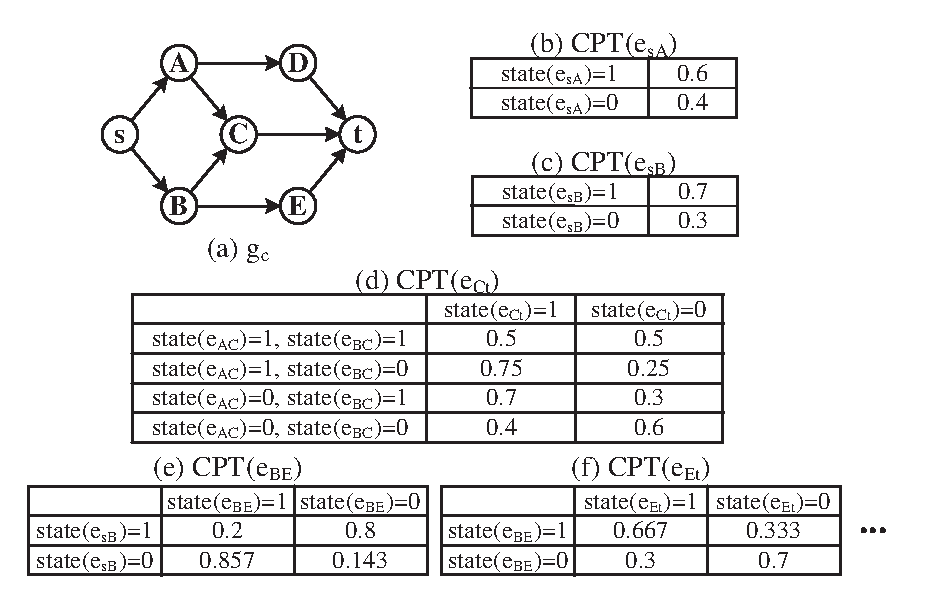
\includegraphics[width=0.9\textwidth]{fig-cpt.eps}
\vspace{-0.3cm}
\caption{\small{Uncertain Graph Model}}
\vspace{-0.4cm}
\end{figure}

\vspace{-0.3cm}
\end{example}

This correlated uncertain graph model can be used in road network to show the fluency correlationship among neighbor roads. For example, in Fig.~\ref{fig:CPT}(a), road $e_{Ct}$ is more possible to be fluent (i.e., $e_{Ct}$ exists) if both the roads $e_{AC}$ and $e_{BC}$ are fluent (i.e., $e_{AC}$ and $e_{BC}$ both exist). Besides, if this model is used in website society, for example, in Fig.~\ref{fig:CPT}(a), if a user visit a website $A$ from its similar website $s$, he is more probable to continue visit its another similar website $C$ or $D$ than not to visit them. These correlationships can only be presented by our correlated uncertain graph model other than the existing independent one.

Given the above uncertain graph model, how to calculate the probability of a \emph{possible world graph}? This would apply the following definition of \emph{Conditional Independent}.

\begin{definition}[Conditional Independent]
  \label{def:conindep}
  $X$, $Y$, $Z$ are three sets of random variables. $Y$ is conditionally independent of $Z$ given $X$ (denoted as $Y\bot Z|X$) in distribution $Pr$ if $\forall$ $x\in X$, $y\in Y$ and $z\in Z$, that is,
  \vspace{-0.2cm}
  \begin{eqnarray*}
   Pr(Y=y,Z=z|X=x) =Pr(Y=y|X=x)\times Pr(Z=z|X=x)
   \vspace{-0.2cm}
  \end{eqnarray*}
\end{definition}

From Definition~\ref{def:conindep}, the probability of a \emph{possible world graph} $g$ equals to
\vspace{-0.2cm}
\begin{equation}
\label{eq:pos-gra-pro}
Pr(g)=\prod_{1\leq i\leq m} CPr(state(e_i))
\vspace{-0.2cm}
\end{equation}
where $m$ is the number of edges in a graph.

For example, the probability of $g_c$ shown in Fig.~\ref{fig:CPT}(a) equals to
\vspace{-0.2cm}
{\setlength\arraycolsep{1pt}
\small
\begin{eqnarray}
\label{eq:egSPr}
\ & Pr(g_1) & = CPr(state(e_{sB})=1) \times CPr(state(e_{BE})=1) \times \cdots{}
\nonumber \\
&&{} =Pr(state(e_{sB})=1) \times Pr(state(e_{BE})=1) | state(e_{sB})=1) \times \cdots {}
\nonumber \\
&&{} = 0.7 \times 0.2 \times \cdots
\end{eqnarray}}

\vspace{-0.9cm}
\subsection{Problem Statement}
\label{sec:sec:pro-state}
\vspace{-0.2cm}

\begin{definition}[Shortest Path Probability ($SPr$)]
\label{def:SPr}
For any path $P$ of $g_c$, the probability of the event that $P$ is the shortest path in the uncertain graph $\mathcal{G}(g_c(V,E,W),Pr)$ is called its Shortest Path Probability, which is calculated as
\vspace{-0.2cm}
\begin{equation}
\label{eq:SPr}
SPr(P)=\sum_{\textrm{$P$ is the shortest path in $g_i$ ($1\leq i\leq n$)}} Pr(g_i)
\vspace{-0.2cm}
\end{equation}
\end{definition}

\vspace{-0.3cm}
\begin{definition}[Threshold-based Shortest Path Query]
  \label{def:ProThre}
Given a correlated uncertain graph $\mathcal{G}(g_c(V,E,W),Pr)$, two vertices $s,t\in V$, and a probabilistic threshold $\tau$, the threshold-based shortest path query returns a path set $SP=\{P_1,P_2,\ldots,P_n\}$ in which each path $P_i$ has a $SPr(P_i)$ larger than the threshold $\tau$.
\vspace{-0.3cm}
\end{definition}

Apparently, if we want to quickly answer the \emph{threshold-based shortest path query}, we have to efficiently calculate the $SPr$. However, the calculation of $SPr$ under the correlated uncertain graph model is \#P-hard. This is because calculating the reachability probability under the independent uncertain graph model is \#P-complete~\cite{jin2011distance}\cite{valiant1979complexity}. When considering the correlation among edges, the calculation of the reachability probability under our model will be harder, whose complexity is at least \#P-complete. Apparently, the calculation of the shortest path probability under our model is even harder than calculating the reachability probability. So our problem is at least \#P-complete, which is \#P-hard.

\vspace{-0.3cm}
\section{Baseline Sampling Algorithm}
\label{sec:base}
\vspace{-0.3cm}

As discussed in the last section, calculating $SPr$ is a \#P-hard problem, so there is no exact solution in polynomial time unless P=NP. Thus, in the rest of this paper, we use sampling methods to get an approximate result. In this section, we give a baseline sampling method based on \emph{Monte Carlo} theory.

During the sampling process, we sample $N$ \emph{possible world graphs}, $G_1$, $G_2$, $\dots$, $G_N$, according to the \emph{pmf} of each edge. Then, on each sampled possible world graph, we run a shortest path algorithm over deterministic graphs to find out its shortest path. Finally, we set a flag $y_{P_i}$ for each path, so that
\vspace{-0.2cm}
\[
y_{P_i}=\left\{ \begin{array}{ll}
1 & \textrm{if $P_i$ is the shortest path in the sampled \emph{possible world graph}}\\
0 & \textrm{otherwise}
\end{array} \right.
\vspace{-0.2cm}
\]
Thus, the estimator $\widehat{SPr_B}$ equals to,
\vspace{-0.2cm}
\begin{equation}
\label{eq:SPrB}
  SPr_B\approx\widehat{SPr_B}=\frac{\sum_{i=1}^Ny_{P_i}}{N}
\vspace{-0.2cm}
\end{equation}

For any sampling method, The \emph{Mean Square Error} \emph{(MSE)} incorporates both the bias and the precision of an estimator into a measure of overall accuracy. It is calculated as,
\vspace{-0.2cm}
\[
MSE(\widehat{\theta})=E[(\widehat{\theta}-\theta)^2]=Var(\widehat{\theta})+Bias(\widehat{\theta},\theta)
\vspace{-0.2cm}
\]

The bias of an estimator is given by,
\vspace{-0.2cm}
\[
Bias(\widehat{\theta})=E(\widehat{\theta})-\theta
\vspace{-0.2cm}
\]
An estimator of $\theta$ is unbiased if its bias is $0$ for all values of $\theta$, that is, $E(\widehat{\theta})=\theta$
As the estimator of \emph{Monte Carlo} method is unbiased~\cite{fishman1991monte}, thus,

\vspace{-0.4cm}
{\setlength\arraycolsep{2pt}
\begin{eqnarray}
\label{eq:VarSPrB}
  MSE(\widehat{SPr_B}) = Var(\widehat{SPr_B}) =\frac{1}{N}SPr_B(1-SPr_B)\approx\frac{1}{N}\widehat{SPr_B}(1-\widehat{SPr_B})
\vspace{-0.4cm}
\end{eqnarray}
}

\vspace{-0.4cm}
The pseudo code is shown in Algorithm~\ref{alg:baseline}.

\vspace{-0.6cm}
\begin{algorithm}[htbp]
  \small{
  \caption{\small{Baseline Algorithm}}
  \label{alg:baseline}
  \KwIn{Start Point $s$, Termination Point $t$}
  \KwOut{$\widehat{SPr_B}$, $Var(\widehat{SPr_B})$}
  \For {$i$ from 1 to $N$}{\label{code:s1s}
    \emph{Sample a possible graph}\;
    $Dijkstra$(\emph{PossibleGraph} $PG$)\;
    $C_{P_i}$++\; {\tcp{to count the number of 1 in $y_{P_i}$}}
  }\label{code:s1e}
  return $(\widehat{SPr_B},Var(\widehat{SPr_B}))$ according to formula~(\ref{eq:SPrB}) and~(\ref{eq:VarSPrB})\;}
\end{algorithm}
\vspace{-0.6cm}

If the sampling number $N$ is far smaller than the number of \emph{possible world graphs}, the \emph{Baseline Sampling Algorithm} is more efficient than the naive exact method discussed in Section~\ref{sec:intro}. But as a consequence, the calculation result is less accurate. According to our experiment result in Section~\ref{sec:exp}, if we want to get a more accurate result, we need to spend many hours to calculate the result using the \emph{Baseline Sampling} algorithm. Whereas, if we want to quickly access the result in seconds, the error may be as large as more than 20\%.

The total time cost $t_{total}$ of the sampling algorithm equals to $t_{total}=t_{once}\times N$ ($t_{once}$ is the time cost in one sampling). \textbf{So, there are two bottlenecks we need to break. The first one is how to get a more accurate result using a smaller sampling size (reduce $N$). The other one is whether we can reduce the time cost in one sampling (reduce $t_{once}$).} Taking the above consideration, we propose an improved sampling method based on \emph{Unequal Probability Sampling}.

\vspace{-0.4cm}
\section{Improved Sampling Algorithm}
\label{sec:impro-samp}
\vspace{-0.2cm}

In this section, we first introduce some knowledge on \emph{Unequal Probability Sampling} in Section~\ref{sec:sec:unequl-pro-samp}. Then, in Section~\ref{sec:sec:DijSampling}, we illustrate our improved sampling algorithm, which is called \emph{DijSampling} algorithm.

\vspace{-0.4cm}
\subsection{Unequal Probability Sampling}
\label{sec:sec:unequl-pro-samp}

\vspace{-0.2cm}
Unequal probability sampling is when some units in the population have probabilities of being selected from others. Suppose a sample of size $N$ is selected randomly from a population $S$ but that on each draw, unit $i$ is sampled according to any probability $q_i$, where $\sum_{i=1}^{S}q_i=1$~\cite{Sampling3rd}. Let $y_i$ be the response variable measured on each unit selection, i.e.,
\vspace{-0.2cm}
\[
y_i=\left\{ \begin{array}{ll}
1 & \textrm{if $i$ is selected in one sampling}\\
0 & \textrm{otherwise}
\end{array} \right.
\vspace{-0.2cm}
\]
Note that if a unit is selected more than once, it is used as many times as it is selected.

There are two classical unbiased estimators, \emph{Hansen-Hurwitz} (\emph{H-H}) and \emph{Horvitz-Thompson} (\emph{H-T}) in unequal probability sampling method. The \emph{H-H} estimator is for random sampling with replacement, while the \emph{H-T} estimator is a more general estimator, which can be used for any probability sampling plan, including both sampling with and without replacement~\cite{Sampling3rd}. For \emph{H-H} estimator, an unbiased estimator of the population total $\xi=\sum_{i=1}^Sy_i$ is given by
\vspace{-0.3cm}
\[
\hat{\xi_q}=\frac{1}{N}\sum_{i=1}^N\frac{y_i}{q_i}
\vspace{-0.3cm}
\]
The variance of \emph{H-H} estimator is
\vspace{-0.4cm}
\[
\widehat{Var}(\hat{\xi_q})=\frac{1}{N(N-1)}\sum_{i=1}^Nq_i(\frac{y_i}{q_i}-\hat{\xi_q})^2
\vspace{-0.3cm}
\]
For \emph{H-T} estimator, the population total $\xi=\sum_{i=1}^Sy_i$ is estimated by
\vspace{-0.3cm}
\[
\hat{\xi_\pi}=\frac{1}{d}\sum_{i=1}^N\frac{y_i}{\pi_i}
\vspace{-0.3cm}
\]
where $\pi_i$ is the probability that the $i^{th}$ unit of the population is included in the sample (\emph{inclusion probability}), and $d$ is the distinct unit number in the sample, which is called \emph{effective sample size}. In addition, the variance of \emph{H-T} estimator is,
\vspace{-0.3cm}
\[
\widehat{Var}(\hat{\xi_\pi})=\sum_{i=1}^d(\frac{1-\pi_i}{\pi_i^2})y_i^2+\sum_{i=1}^d\sum_{j=1,j\neq i}^d(\frac{\pi_{ij}-\pi_i\pi_j}{\pi_i\pi_j})\frac{y_iy_j}{\pi_{ij}}
\vspace{-0.3cm}
\]
where $\pi_{ij}$ is the \emph{joint inclusion probability} of units $i$ and $j$ (the probability that $i$ and $j$ are sampled at the same time).

As both of the above estimators are unbiased, i.e., $Bias(\widehat{\theta},\theta)=0$, the variance can be used to evaluate the accuracy of the estimators.

\vspace{-0.2cm}
\subsection{\emph{DijSampling Algorithm}}
\label{sec:sec:DijSampling}
\vspace{-0.1cm}

Reviewing the two bottlenecks in Section~\ref{sec:base}, the underlying cause of the first one is that the \emph{Baseline Sampling} algorithm only samples one instance of the sample space in one sampling. \textbf{We consider a method to sample a lot of \emph{possible world graphs} together in one sampling in order to reduce $N$}. Then, for the second bottleneck, when sampling once, the \emph{Baseline Sampling} algorithm samples the whole \emph{possible world graph}, and the followed \emph{Dijkstra} algorithm is run on the whole \emph{possible world graph}. Thus, \textbf{we should think of a method that only samples a part of a \emph{possible world graph} each time to reduce $t_{once}$}. These are the main purposes of our \emph{DijSampling} algorithm. We use an example to explain these advantages in detail.

\begin{example}[Advantages of Improved Sampling Algorithm]
\label{eg:imp-samp-adv}
Fig.~\ref{fig:imp-samp-adv} shows 4 \emph{possible world graphs}. These \emph{possible world graphs} have the same shortest path, $P_{sBEt}$. (Actually, there are 16 such \emph{possible world graphs}, and we only show 4 of them.) We apply shortest path algorithm to sample edges $e_{sB}$, $e_{BE}$, and $e_{Et}$, and the 16 \emph{possible world graphs} are totally the \emph{possible world graphs} that contain $P_{SBEt}$ as the shortest path. Thus, our \emph{DijSampling} algorithm only needs one sampling and can sample all these 16 \emph{possible world graphs} together. But in \emph{Baseline Sampling} algorithm, it takes 16 times to sample them.  In other words, sampling once in \emph{DijSampling} algorithm has the same effect with sampling 16 times in \emph{Baseline Sampling}. If the \emph{Baseline Sampling} needs 1600 times of sampling to get an accurate result, the \emph{DijSampling} algorithm only needs 100 times of sampling. Thus, by together sampling the \emph{possible world graphs} containing the same shortest path, the \emph{DijSampling} algorithm can effectively reduce the sample size $N$. Moreover, since the 4 edges, $e_{AC}$, $e_{AD}$, $e_{Ct}$ and $e_{Dt}$, are not sampled in one sampling of \emph{DijSampling} algorithm, the \emph{DijSampling} algorithm has a smaller $t_{each}$ than the \emph{Baseline Sampling} algorithm.

\begin{figure}[htbp]
\vspace{-0.6cm}
\label{fig:imp-samp-adv}
\centering
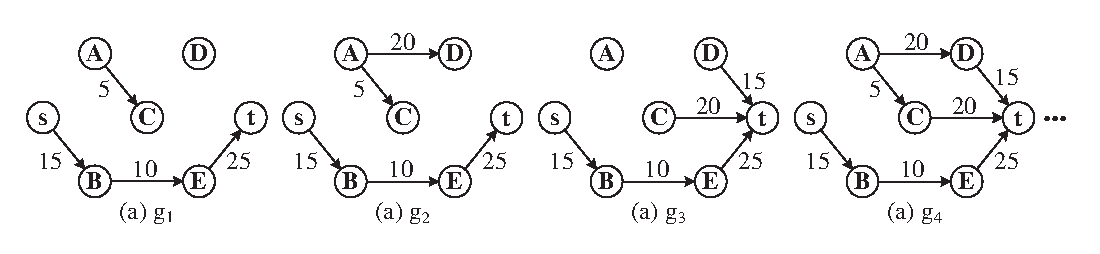
\includegraphics[width=0.99\textwidth]{fig-imp-sample-adv.eps}
\vspace{-0.3cm}
\caption{\small{Possible World Graphs in which $P_{sBEt}$ is the shortest path}}
\vspace{-0.4cm}
\end{figure}

\vspace{-0.3cm}
\end{example}

As indicated in the above example, the main idea of our \emph{DijSampling} algorithm is to sample the edges at the same time with the process of \emph{Dijkstra} algorithm. The pseudo-code is shown in Algorithm~\ref{alg:DijSampling}. The \emph{DijSampling} is proceeded during the process of \emph{Dijkstra} algorithm. When the \emph{Dijkstra} algorithm needs the messages of an edge such as its existence or weight, we sample it according to its \emph{pmf} (Line~\ref{code:samp-edge}). Note that if this edge is outgoing the source query point $s$, we need to determine whether its in-degree is zero. If it is so ($s=s_z$), we just sample it according to its \emph{pmf} (Line~\ref{code:samp-edge-zero}). Otherwise (Line~\ref{code:samp-edge-nonzero}), we sample this edge with the probability estimated by the following formula

\vspace{-0.3cm}
\begin{equation}
\small{
\label{eq:margin}
Pr(state(e_s)=1)=\frac{\sum_{1\leq i\ldots\leq m_{in}; k=0,1}CPr(state(e_s)=1|state(e_i)=k,\cdots)}{\sum_{1\leq i\ldots\leq m_{in}; k=0,1}CPr(state(e_s)=k|state(e_i)=k,\cdots)}
}
\end{equation}

This formula means we sample the edge $e_s$ using the average probability when $state(s)=1$ in its \emph{CPT} as its existence probability, while using the average probability when $state(s)=0$ as its nonexistence probability. The reason why we treat the $e_s$ specially will be explained latter in this subsection.

The following is an example illustrating the process of \emph{DijSampling} algorithm.

\begin{algorithm}[htbp]
  \small{
  \caption{\small{DijSampling Algorithm}}
  \label{alg:DijSampling}
  \KwIn{Start Point $s$, Termination Point $t$, sampling times $N$}
  \KwOut{\scriptsize{$\widehat{SPr_{H-H}}$, $Var(\widehat{SPr_{H-H}})$, $\widehat{SPr_{H-T}}$, $Var(\widehat{SPr_{H-T}})$}}
  \For {$i$ from $1$ to $N$}
  {
     running \emph{Dijkstra} \Begin{
     \If {\emph{Dijkstra} needs the messages of an edge}
     {
       \label{code:samp-edge}
       \If{$s$==$s_z$}
       {
         Sample the edges outgoing $s$ according to their \emph{CPT}s \; \label{code:samp-edge-zero}
       }
       \Else
       {
         Sample the edges outgoing $s$ according to formula~(\ref{eq:margin}) \; \label{code:samp-edge-nonzero}
       }
       Sample the other edges according to their \emph{CPT}s \;
     }
     \Else
     {
       continue the \emph{Dijkstra} algorithm \;
     }

     return (result shortest path $P_i$) \;
  }
  $y_{P_i}$++ \;
  }
  calculate \scriptsize{$\widehat{SPr_{H-H}}$, $Var(\widehat{SPr_{H-H}})$, $\widehat{SPr_{H-T}}$, $Var(\widehat{SPr_{H-T}})$}\;
}
\end{algorithm}
\vspace{-0.6cm}

\begin{example}
\label{eg:sampling}

Fig.~\ref{fig:sampling} shows the process of \emph{DijSampling} algorithm. In this figure, we use dashed lines to denote the unsampled edges, solid lines to denote the existing edges after sampling, and no lines (empty) to denote the nonexisting edges after sampling. Specifically, Fig.~\ref{fig:sampling}(a) is the $g_c$ of the uncertain graph in Fig.~\ref{fig:CPT} before sampling, and Fig.~\ref{fig:sampling}(b)-(d) are the graphs after sampling the designated edges.

Assume the start query point is $s$ and terminal query point is $t$. We first sample $e_{sA}$ and $e_{sB}$ according to Fig.~\ref{fig:CPT}(b) and Fig.~\ref{fig:CPT}(c) respectively. For example, we sample the $e_{sB}$ with probability 0.7 existing and 0.3 nonexisting. After that, we assume that $e_{sA}$ does not exists and $e_{sB}$ exists (Fig.~\ref{fig:sampling}(b)). Then, we sample edge $e_{BE}$ and $e_{BC}$. For example, for edge $e_{BE}$, as we have sampled edge $e_{sB}$ exists, then $state(e_{sB})=1$. So we sample $e_{BE}$ with probability 0.2 existing, and probability 0.8 nonexisting (Fig.~\ref{fig:sampling}(c)). Repeat the above process, after we sample to Fig.~\ref{fig:sampling}(d), we can know $P_{sBEt}$ is the shortest path. Thus, there is no need to sample the other edges (dashed edges in Fig.~\ref{fig:sampling}(d)).

\vspace{-0.6cm}
\begin{figure}[htbp]
\centering
  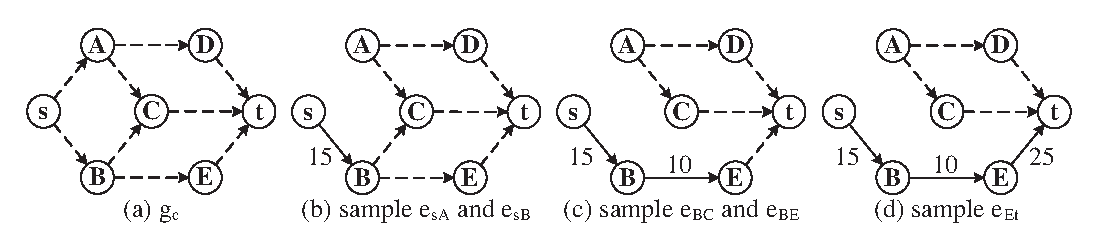
\includegraphics[width=0.99\textwidth]{fig-sample.eps}
\vspace{-0.5cm}
  \caption{\small{\emph{DijSampling} Process}}
  \label{fig:sampling}
\vspace{-0.7cm}
\end{figure}

In addition, if the query is $B$ to $t$ instead, the first edges should be sampled are $e_{BE}$ and $BC$. The sampling existence probability of $e_{BE}$ is $(0.2+0.857)/(0.2+0.857+0.8+0.143)=0.5285$, and similarly the nonexistence probability is $0.4715$. Then, the remained sampling steps are the same with those mentioned above (from $s$ to $t$).

\vspace{-0.2cm}
\end{example}

After describing the algorithm, let us see how to estimate the $SPr$s. According to Section~\ref{sec:sec:unequl-pro-samp}, the \emph{H-H} estimator of $SPr$ can be calculated as

\vspace{-0.3cm}
\begin{equation}
\label{eq:HHSPr}
SPr_{H-H}\approx\widehat{SPr_{H-H}}=\frac{1}{N}\sum_{i=1}^N\frac{Pr_{P_i}y_{P_i}}{q_i}
\vspace{-0.2cm}
\end{equation}
where $N$ is the sampling times, and $Pr_{P_i}$ is the probability of the sampled \emph{possible world graph} that $P_i$ is the shortest path in it, which can be calculated as

\vspace{-0.2cm}
\begin{equation}
\label{eq:pos-gra-pro}
Pr_{P_i}=\prod_{1\leq i\leq m_{samp}} CPr(state(e_i))
\vspace{-0.2cm}
\end{equation}
where $m_{samp}$ is the number of sampled edges in one sampling process.

The variance of this estimator equals to
\vspace{-0.4cm}
\begin{equation}
\label{eq:HHVar}
Var(\widehat{SPr_{H-H}})=\frac{1}{N(N-1)}\sum_{i=1}^Nq_i(\frac{Pr_{P_i}}{q_i}-\widehat{SPr_{H-H}})^2
\vspace{-0.3cm}
\end{equation}

When $q_i=Pr_{P_i}$, i.e., we sample each edge according to its \emph{pmf}~\cite{jin2011distance}, it has been proved that, the variance in formula~(\ref{eq:HHVar}) is minimum. At this moment, the $\widehat{SPr_{H-H}}$ in formula~(\ref{eq:HHSPr}) equals to
\vspace{-0.2cm}
\begin{equation}
\label{eq:minHHSpr}
min(\widehat{SPr_{H-H}})=\frac{\sum_{i=1}^Ny_{P_i}}{N}
\vspace{-0.2cm}
\end{equation}
and its corresponding variance is
\vspace{-0.2cm}
\begin{equation}
\label{eq:minHHVar}
min(Var(\widehat{SPr_{H-H}}))=\frac{1}{N}\widehat{SPr_{H-H}}(1-\widehat{SPr_{H-H}})
\vspace{-0.1cm}
\end{equation}

The \emph{H-H} estimator and its variance equals to those of the baseline algorithm.

Similarly, we give the formula to compute \emph{H-T} estimator. Suppose, in the $N$ times sampling, there are $v$ different sampling results. Thus the probability that each one of the $v$ results may be sampled is $\pi_i=1-(1-q_i)^N$. So the estimator $\widehat{SPr_{H-T}}$ is,

\vspace{-0.1cm}
\begin{equation}
  \label{eq:SPrHT}
  SPr_{H-T}\approx\widehat{SPr_{H-T}}=\frac{1}{N}\sum_{i=1}^N\frac{Pr_{P_r} y_{P_i}}{\pi_i}
\vspace{-0.1cm}
\end{equation}
This estimator is unbiased as well \cite{jin2011distance}\cite{Sampling3rd}. $\pi_{ij}=1-(1-q_i)^n-(1-q_j)^N-(1-q_i-q_j)^N$ is the probability that $\pi_i$ and $\pi_j$ are in the result set at the same time, and the variance of this estimator is,

\vspace{-0.2cm}
\begin{eqnarray}
\label{eq:VarSPrHT}
  \ & Var(\widehat{SPr_{H-T}}) & = \sum_{i\in v}(\frac{1-\pi_i}{\pi_i})(Pr_{P_i})^2 +\sum_{\substack{i,j\in v, i\neq j}}(\frac{\pi_{ij}-\pi_i\pi_j}{\pi_i\pi_j})Pr_{P_j} Pr_{P_j}
\end{eqnarray}

\vspace{-0.2cm}
Again, when $q_i=Pr_{P_i}$, $Var(\widehat{SPr_{H-T}})$ gets its minimum value. However, at this time, $\widehat{SPr_{H-T}}\neq\widehat{SPr_B}$. Moreover, $Var(\widehat{SPr_{H-T}})\leq Var(\widehat{SPr_B})$ \cite{jin2011distance}.

\vspace{-0.2cm}
\subsubsection{The Special $e_s$ in Line~\ref{code:samp-edge-nonzero} of Algorithm~\ref{alg:DijSampling}}

The reason why we treat the $e_s$ specially is that the edges outgoing a vertex always depend its parent edges under the uncertain graph model introduced in Section~\ref{sec:sec:model}. Just like Example~\ref{eg:sampling}, we cannot know the sampling probability of $e_{BE}$ if the state of $e_{sB}$ is unknown. Actually, we can just randomly choose a root vertex and sample from it. After it reach the source query point, we continue our algorithm. However, this method is apparently uneconomical since the long journey before the source query point has no contribution to the result set except for a start probability. Thus, we use formula~(\ref{eq:margin}) to quickly estimate this probability instead.

Our algorithm can achieve $q_i=Pr_{P_i}$ except for this step in Line~\ref{code:samp-edge-nonzero} of Algorithm~\ref{alg:DijSampling}. In this situation, if we still use the estimators with the minimum variance,  they are no longer unbiased. But fortunately, we can prove that this bias is close to zero when the number of sampled edges are large, which is Theorem~\ref{the:bias} in follows.

\vspace{-0.2cm}
\begin{theorem}
\label{the:bias}
The bias of estimators equals nearly to zero when the number of sampled edges are large.
\end{theorem}

\begin{proof}
\label{pro:bias}

\vspace{-1cm}
\begin{figure}[htbp]
\centering
  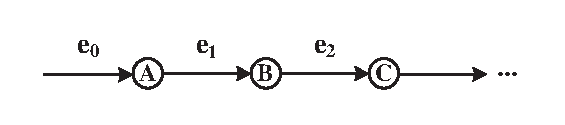
\includegraphics[width=0.5\textwidth]{fig-bias.eps}
\vspace{-0.4cm}
  \caption{\small{\emph{Dependency Schematic Diagram for Derivation of Bias}}}
  \label{fig:bias}
\vspace{-0.6cm}
\end{figure}

We take the situation in which $s$ has only one injection edge as an example to derivate the bias. The derivation when $s$ has more than one injection edges are similar. A schematic diagram is shown in Fig.~\ref{fig:bias}. $e_1$ is the first edge we want to sample. Let $Pr(e_i|e_j)=Pr(state(e_i)=1|state_{e_j}=1)$, $Pr(e_i|\overline{e_j})=Pr(state(e_i)=1|state_{e_j}=0)$, $Pr(\overline{e_i}|e_j)=Pr(state(e_i)=0|state_{e_j}=1)$, and $Pr(\overline{e_i}|\overline{e_j})=Pr(state(e_i)=0|state_{e_j}=0)$, then the real sampling probability of $e_1$ equals to

\vspace{-0.6cm}
{\setlength\arraycolsep{1pt}
\small
\begin{eqnarray}
\label{eq:egSPr}
& Pr(e_1) & = Pr(e_1|e_0) \times Pr(e_0) + Pr(e_1|\overline{e_0}) \times Pr(\overline{e_0}) {}
\nonumber \\
&&{}= Pr(e_1|e_0) \times Pr(e_0) + Pr(e_1|\overline{e_0}) \times (1-Pr(\overline{e_0}))
\vspace{-0.6cm}
\end{eqnarray}}
But our estimated probability of $e_1$ equals to,
\vspace{-0.3cm}
{\setlength\arraycolsep{1pt}
\small
\begin{eqnarray*}
\label{eq:egSPr}
\widehat{Pr(e_1)}=Pr(e_1|e_0)\times\widehat{Pr(e_0)}+Pr(e_1|\overline{e_0})\times(1-\widehat{Pr(\overline{e_0})})
\vspace{-0.4cm}
\end{eqnarray*}}
Thus, the bias after sampling the first edge $Bias^{(1)}$ equals to,
\vspace{-0.3cm}
{\setlength\arraycolsep{1pt}
\small
\begin{eqnarray*}
\label{eq:egSPr}
Bias^{(1)} = \widehat{Pr(e_1)}-Pr(e_1)= (Pr(e_1|e_0)-Pr(e_1|\overline{e_0}))\times(Pr(e_0)-\widehat{Pr(e_0)})
\vspace{-0.3cm}
\end{eqnarray*}}
Similarly, we can get the bias after sampling the second edge,
\vspace{-0.2cm}
{\setlength\arraycolsep{1pt}
\small
\begin{eqnarray*}
\label{eq:egSPr}
& Bias^{(2)} & = \widehat{Pr(e_2)}-Pr(e_2) {} \\
&& {}=(Pr(e_2|e_1)-Pr(e_2|\overline{e_1}))\times (Pr(e_1|e_0)-Pr(e_1|\overline{e_0}))\times(Pr(e_0)-\widehat{Pr(e_0)})
\end{eqnarray*}
\vspace{-0.2cm}}
Recursively, we can get the bias after sampling $m_{sample}$ edges,
{\setlength\arraycolsep{1pt}
\small
\begin{eqnarray*}
\label{eq:egSPr}
& Bias^{(m_{sample})} & = \widehat{Pr(e_{m_sample})}-Pr(e_{m_sample}) {} \\
&& {}=\prod_{i=1}^{m_{sample}}(Pr(e_i|e_j)^{(i)}-Pr(e_i|\overline{e_j})^{(i)})\times(Pr(e_0)-\widehat{Pr(e_0)})
\end{eqnarray*}}
where $Pr(e_i|e_j)^{(i)}$ and $Pr(e_i|\overline{e_j})^{(i)}$ are conditional probabilities of $i^{th}$ sampled edge.

Apparently, $Bias^{(m_{sample})}\rightarrow 0$ when $m_{sample}$ is large enough.~~~~~~~~~~~~~~~~~~~~~~~~~~~$\Box$

\end{proof}

\vspace{-0.4cm}
\section{Performance Evaluations}
\label{sec:exp}
\vspace{-0.2cm}

In this section, we will report and analyze our experiment results. All the experiments are proceeded on a PC with CPU Inter(R) Core(TM)i7-2600, frequency 3.40GHz, memory 8.00GB, hard disk 500GB. The Operation System is Microsoft Windows 7 Enterprise Edition. The development software is Microsoft Visual Studio 2010, using language C++ and its standard template library (STL).

\vspace{-0.3cm}
\subsubsection{The Dataset}
\label{sec:exp:dataset}
\vspace{-0.1cm}

The real data used in this paper can be classified into two categories. One is sparse dataset such as Road Network data\footnote{http://www.cs.utah.edu/~lifeifei/SpatialDataset.htm}, and the other one is Social Network data\footnote{http://snap.stanford.edu/data}. The numbers of vertices and edges are listed in Table~\ref{tab:Rdataset}.

In real datasets, the edges are certain, so we need to change the certain graphs into uncertain graphs. In Road Network Datasets, we use the method which is introduced in~\cite{hua2010probabilistic}. Use Normal Distribution $N(\mu,\sigma)$ to generate the weights on each edge. Here, $\mu$ is the edge weight in original datasets, and $\sigma$ is the variance of the generated weights. $\sigma$ is different according to different edges, which is normally distributed as $N(\mu_\sigma,\sigma_\sigma)$. Here, $\mu_\sigma=xR$, and the value range of $x$ is $[1\%,5\%]$. In default condition, $\mu_\sigma=1\%R$, and $R$ is the value range of all weights in original datasets. In the same way, we generate the weights and probabilities on edges in Social Network datasets.

\begin{table}[htbp]
\vspace{-0.2cm}
  \centering
  \caption{\small{Real Dataset Parameters}}
\vspace{-0.1cm}
  \label{tab:Rdataset}
  \begin{tabular}{|c|c|c|}
    \hline
    \bfseries {Name of Dataset} & \bfseries {Vertex Number} & \bfseries {Edge Number} \\
    \hline
    OLdenburg (OL) Road Network & 6,105 & 7,035 \\
    \hline
    San Francisco Road Network (SF) & 174,956 & 223,001 \\
    \hline
    wiki-Vote & 7,115 & 103,689 \\
    \hline
    %soc-Epinions1 & 75,879 & 508,837 \\
%    \hline
    \end{tabular}
\vspace{-0.4cm}
\end{table}

For all the datasets, we choose 100 pairs of vertices as starting points and termination points. After the 100 tests, we calculate the average time cost, memory cost, \emph{Mean Square Error (MSE)} and relative error as the experiment results. We set the threshold defaulted to be 0.5 and compare the proformance of baseline sampling algorithm (denoted as \emph{BS}) and our improved \emph{DijSampling} algorithm (denoted as \emph{DS}).

\vspace{-0.2cm}

\subsubsection{Running Time}
\label{sec:exp:alg:time}

Fig.~\ref{fig:time} shows the running time vs sample size for the two sampling algorithms on different real datasets. From the results, we can observe that with the increase of sample size, the time cost for the two algorithms all increases. The time cost of \emph{BS} is always largest than that of \emph{DS}. In addition, we observe that the larger the graph is, the more time will be cost.

\begin{figure*}[htbp]
\vspace{-0.7cm}
  \centering
  \subfigure[\small{OL}]{
      \label{fig:time:ol}
      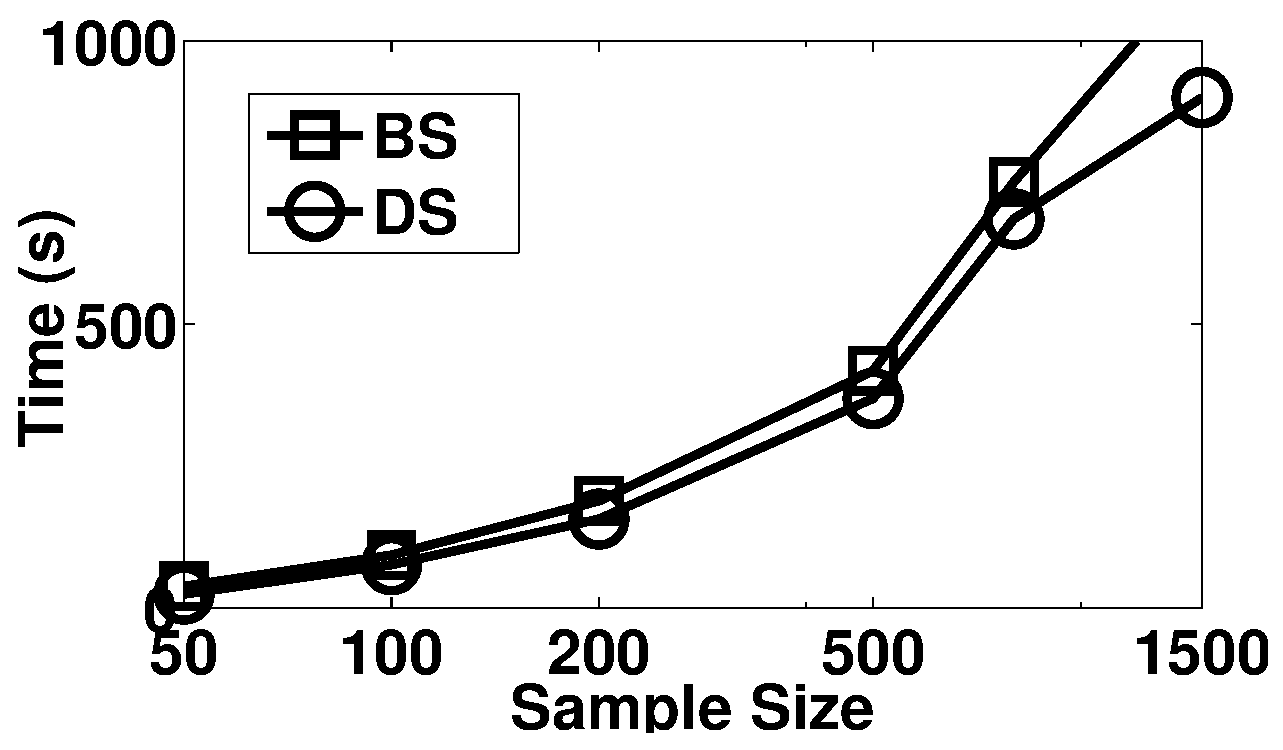
\includegraphics[width=0.32\textwidth]{fig-time-OL.eps}}
  \subfigure[\small{SF}]{
      \label{fig:time:sf}
      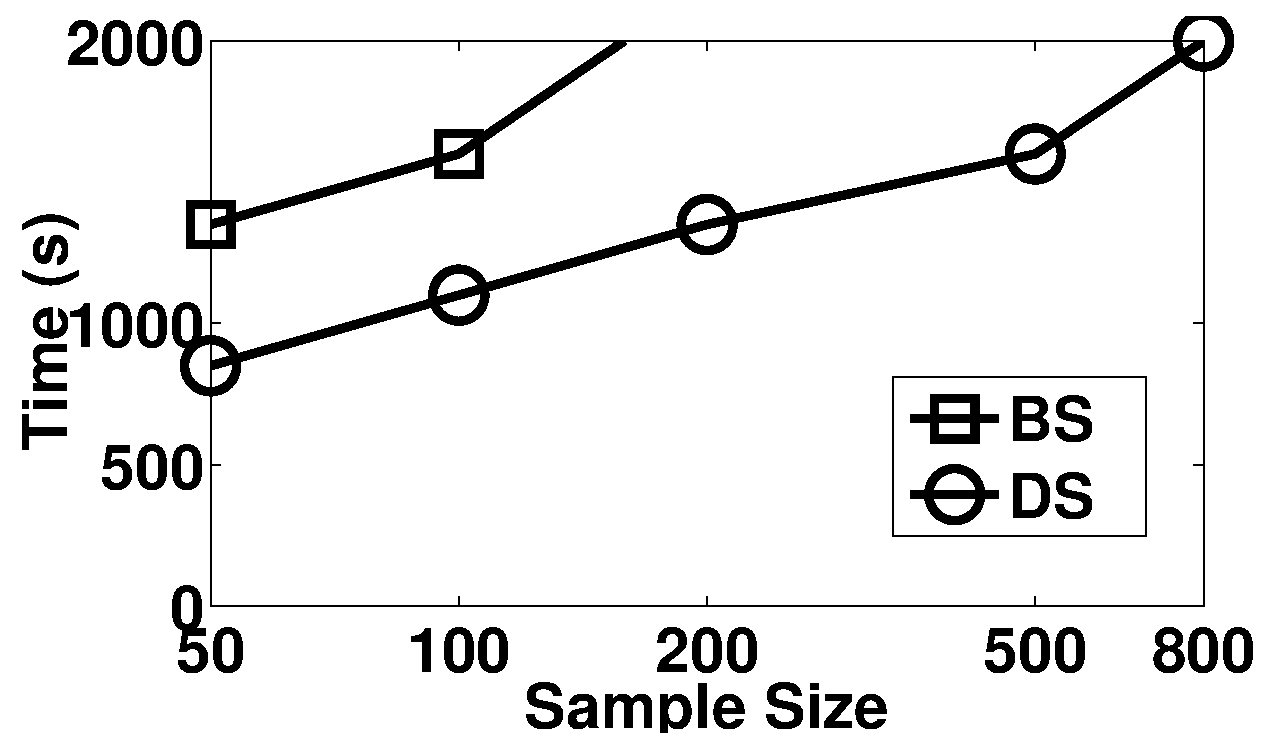
\includegraphics[width=0.32\textwidth]{fig-time-SF.eps}}
  \subfigure[\small{wiki-Vote}]{
      \label{fig:time:wiki}
      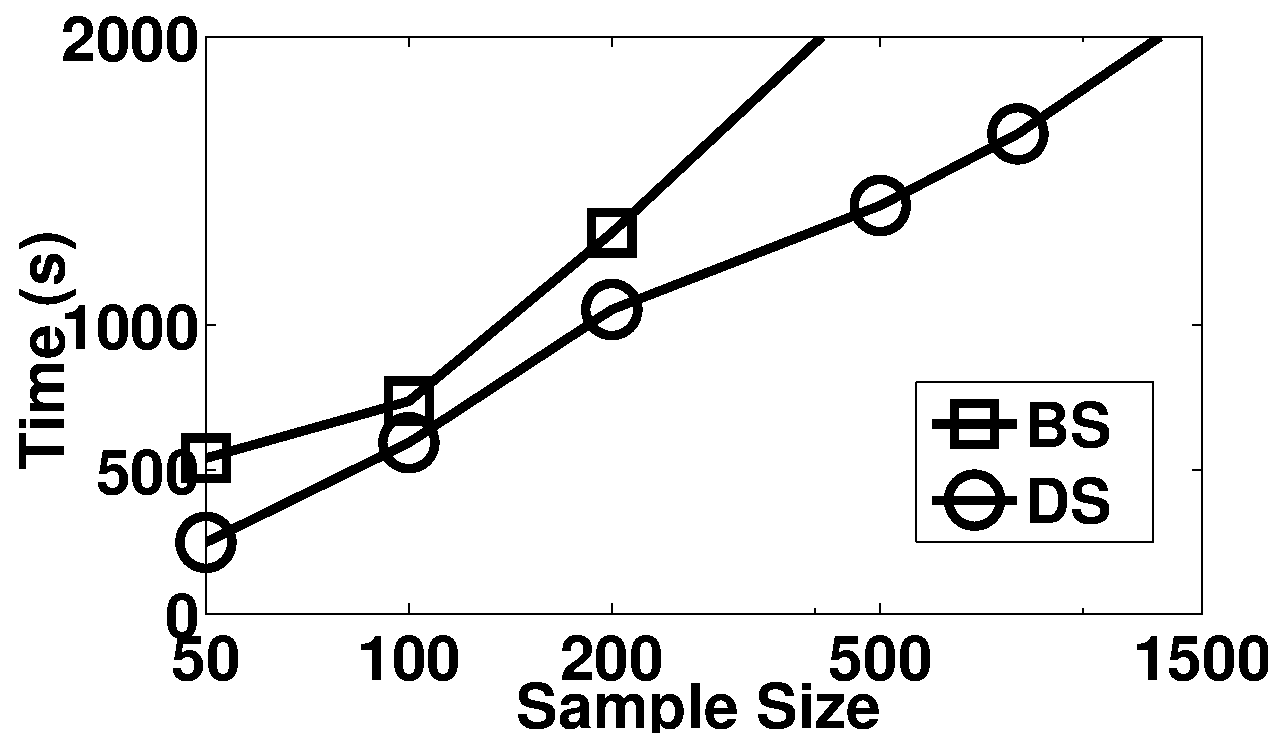
\includegraphics[width=0.32\textwidth]{fig-time-Wiki.eps}}
  %\subfigure[\small{soc-Epinions1}]{
%      \label{fig:time:soc}
%      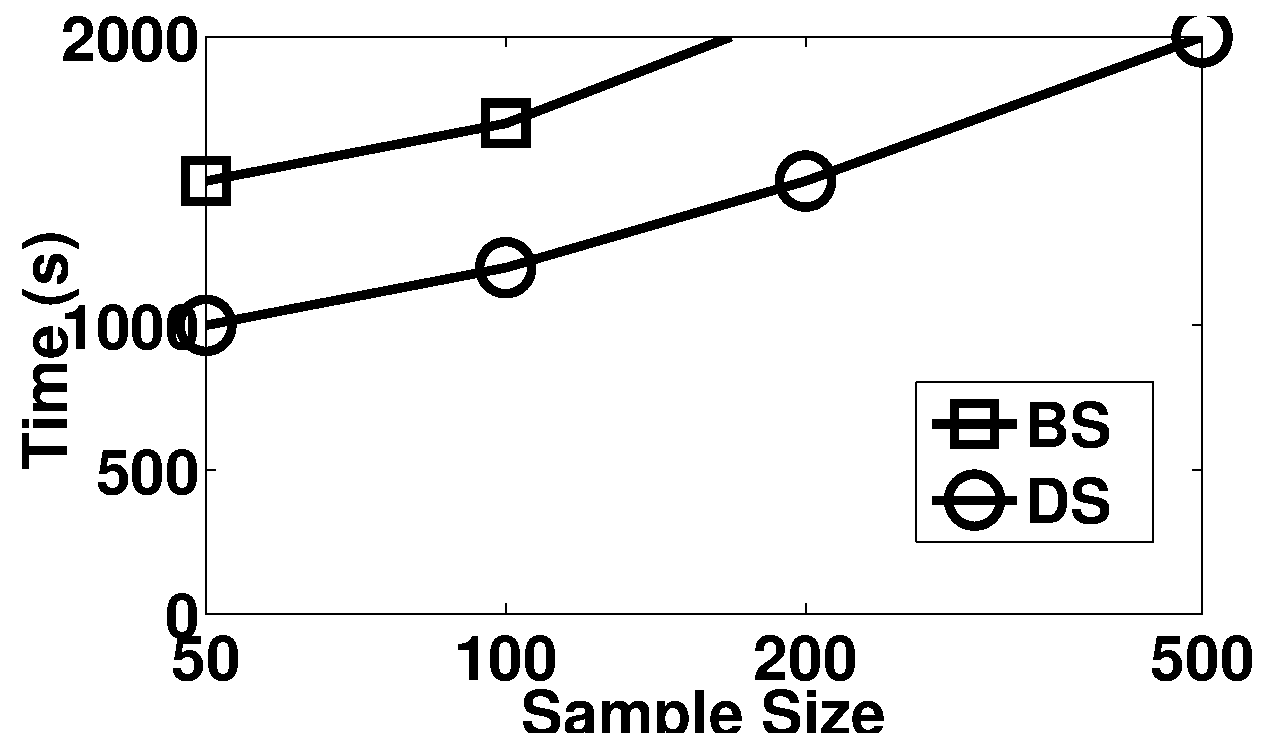
\includegraphics[width=0.35\textwidth]{fig-time-Soc.eps}}
\vspace{-0.3cm}
  \caption{Running time vs Sample Size}
  \label{fig:time}
\vspace{-0.6cm}
\end{figure*}

The results above are reasonable. The running time depends on the number of sampled edges. The more edges sampled, the more time an algorithm will cost. As the \emph{BS} Algorithm samples more edges, the whole possible graph, its running time is longer.


\subsubsection{Memory Cost}
\label{sec:exp:memory}

\begin{figure*}[htbp]
\vspace{-1.1cm}
  \centering
  \subfigure[\small{OL}]{
      \label{fig:memory:ol}
      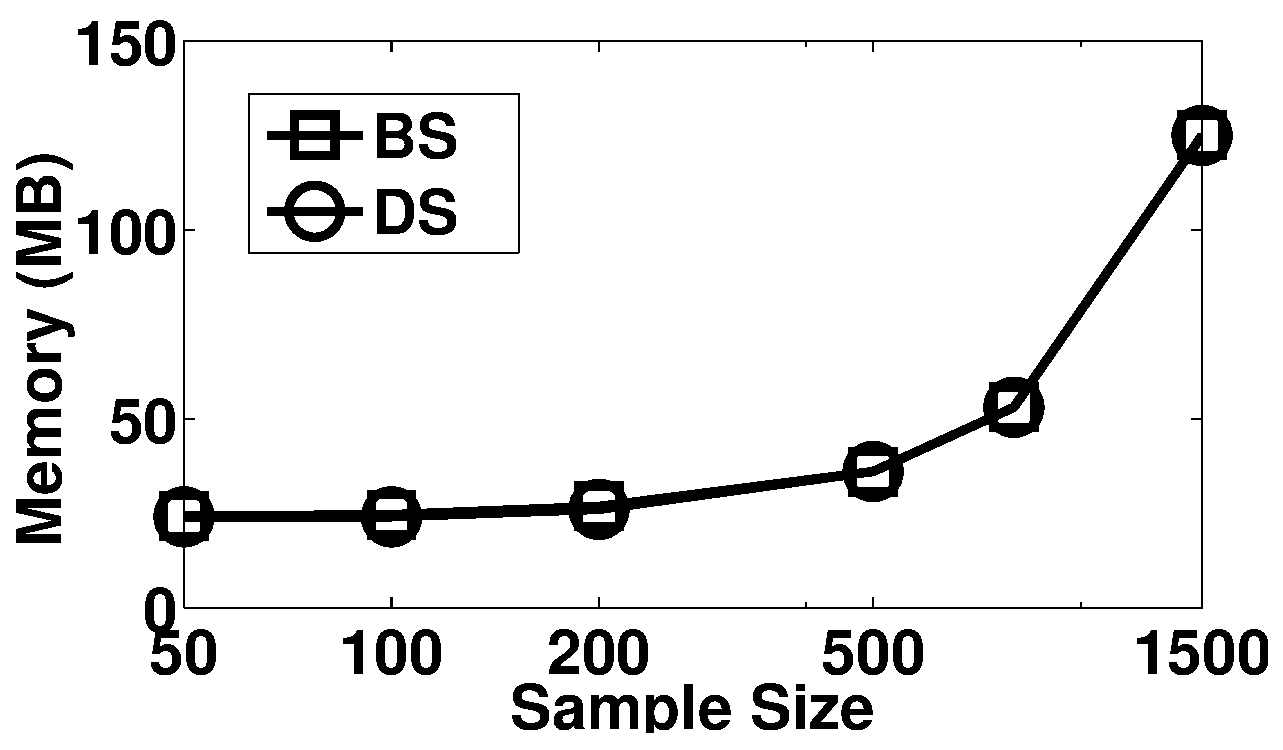
\includegraphics[width=0.32\textwidth]{fig-mem-OL.eps}}
  \subfigure[\small{SF}]{
      \label{fig:memory:sf}
      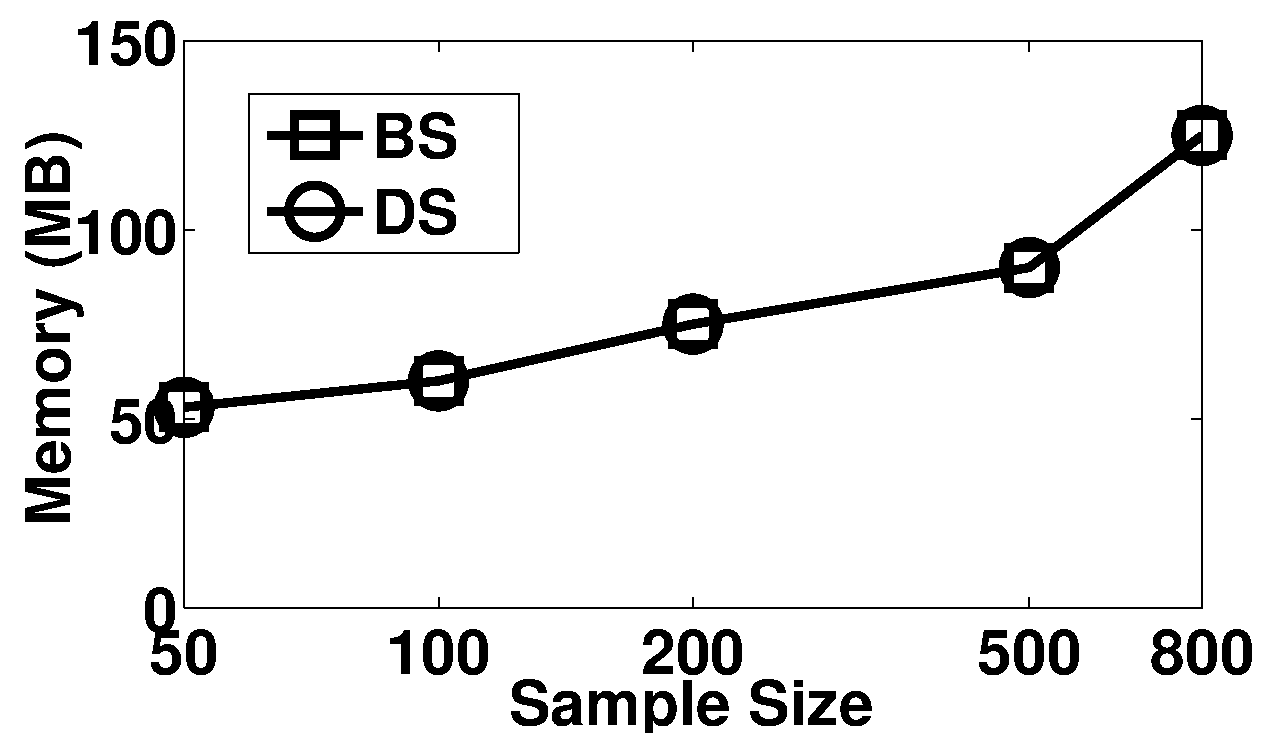
\includegraphics[width=0.32\textwidth]{fig-mem-SF.eps}}
  \subfigure[\small{wiki-Vote}]{
      \label{fig:memory:wiki}
      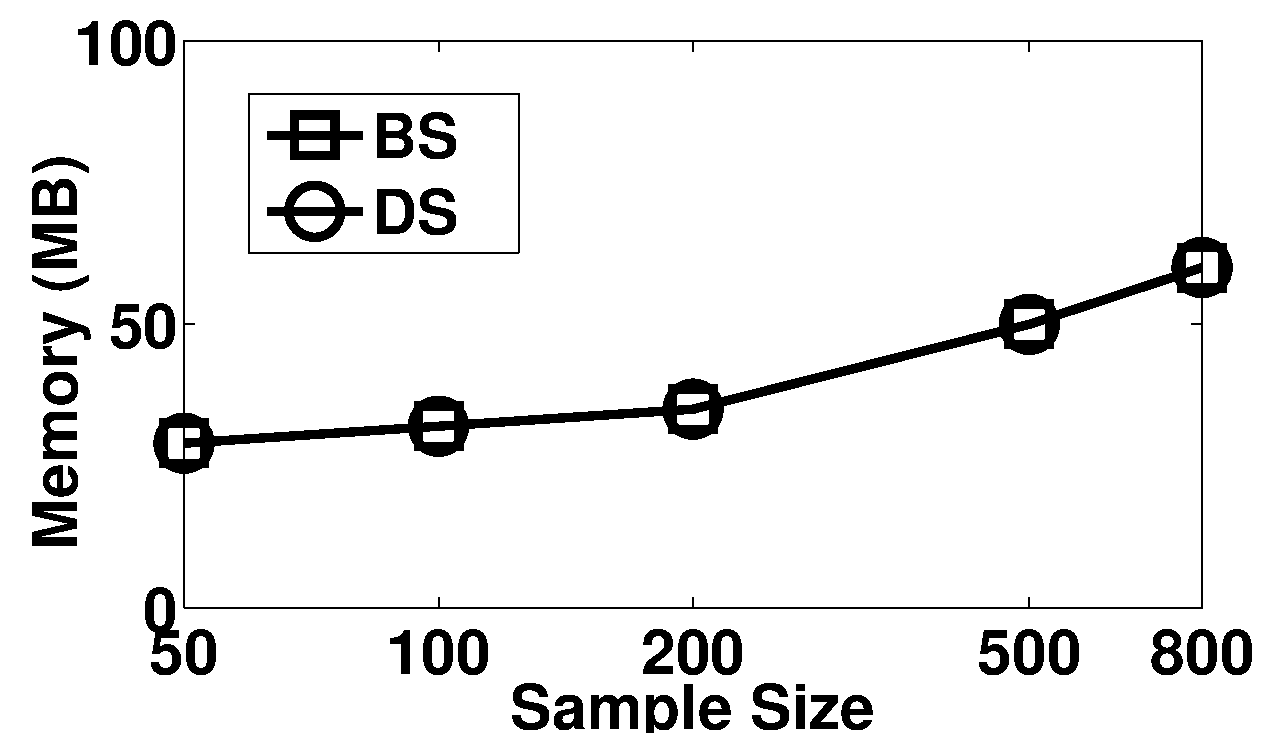
\includegraphics[width=0.32\textwidth]{fig-mem-Wiki.eps}}
  %\subfigure[\small{soc-Epinions1}]{
%      \label{fig:memory:soc}
%      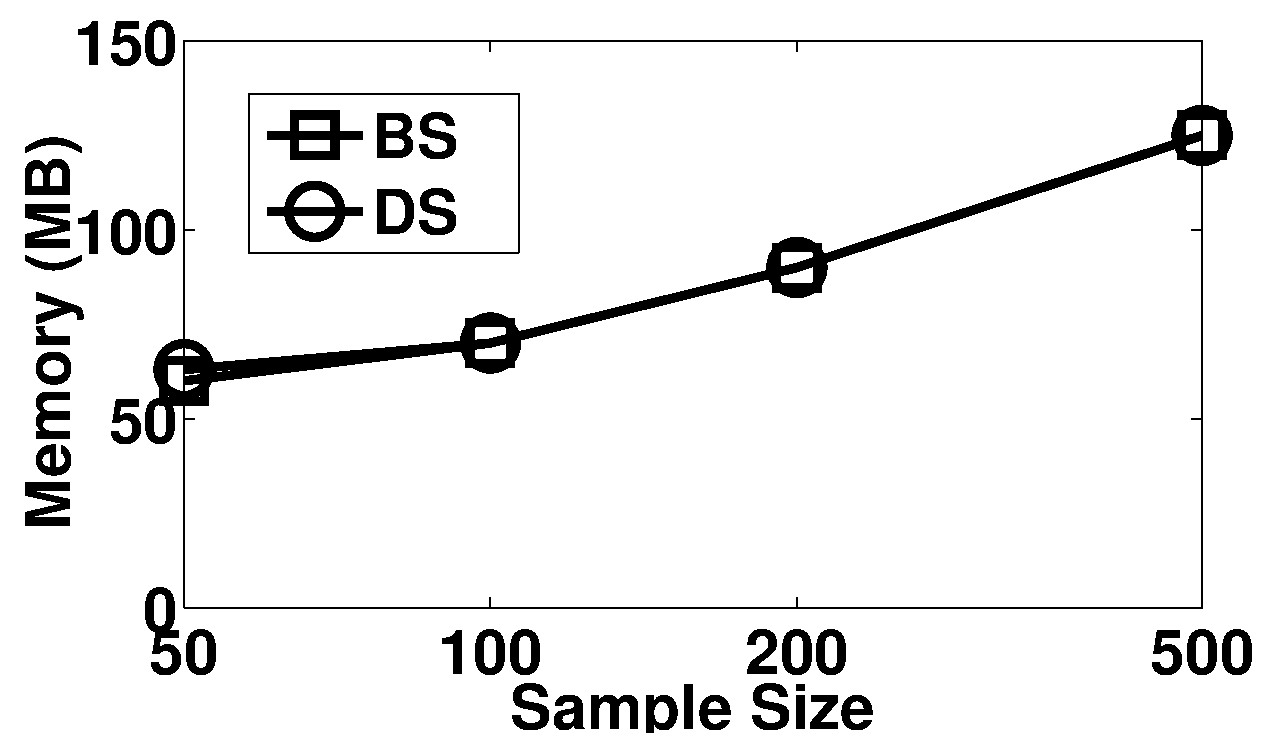
\includegraphics[width=0.4\textwidth]{fig-mem-Soc.eps}}
\vspace{-0.3cm}
  \caption{Memory Cost vs Sample Size}
  \label{fig:memory}
\vspace{-0.6cm}
\end{figure*}

Fig.~\ref{fig:memory} shows the memory cost vs sample size on different datasets. It can be seen that with the increase of sample times, the memory cost of two algorithms increases. The memory cost of the two algorithms is almost the same.

The phenomena above is reasonable that as sample size increases, the program needs to explore more space to find the shortest path and calculate estimator with corresponding variance. Thus, the memory cost increases with the increase of sample times. Moreover, both the algorithms need to save the structures of graph data and some queues for \emph{Dijkstra} algorithm, which are the same. The only difference between the two methods are the flags showing whether each edge is sampled, which takes little memory cost. Thus, the memory cost of the two algorithms is nearly the same.

\vspace{-0.2cm}
\subsubsection{Accuracy}
\label{sec:exp:estim:var}

We test \emph{Mean Square Error (MSE)} and relative error of the estimators to show the accuracy of different algorithms. As the bias caused by formula~(\ref{eq:margin}) is always 0 in the experiment result, we do not show it in our result figures. Since the variance of \emph{BS} estimator is the same as the \emph{H-H} estimator of \emph{DS}, we show them using the same line in result figure. The method of calculating \emph{relative error} is the same as that in~\cite{jin2011distance}.

\begin{figure*}[htbp]
\vspace{-0.7cm}
  \centering
  \subfigure[\small{OL}]{
      \label{fig:mse:ol}
      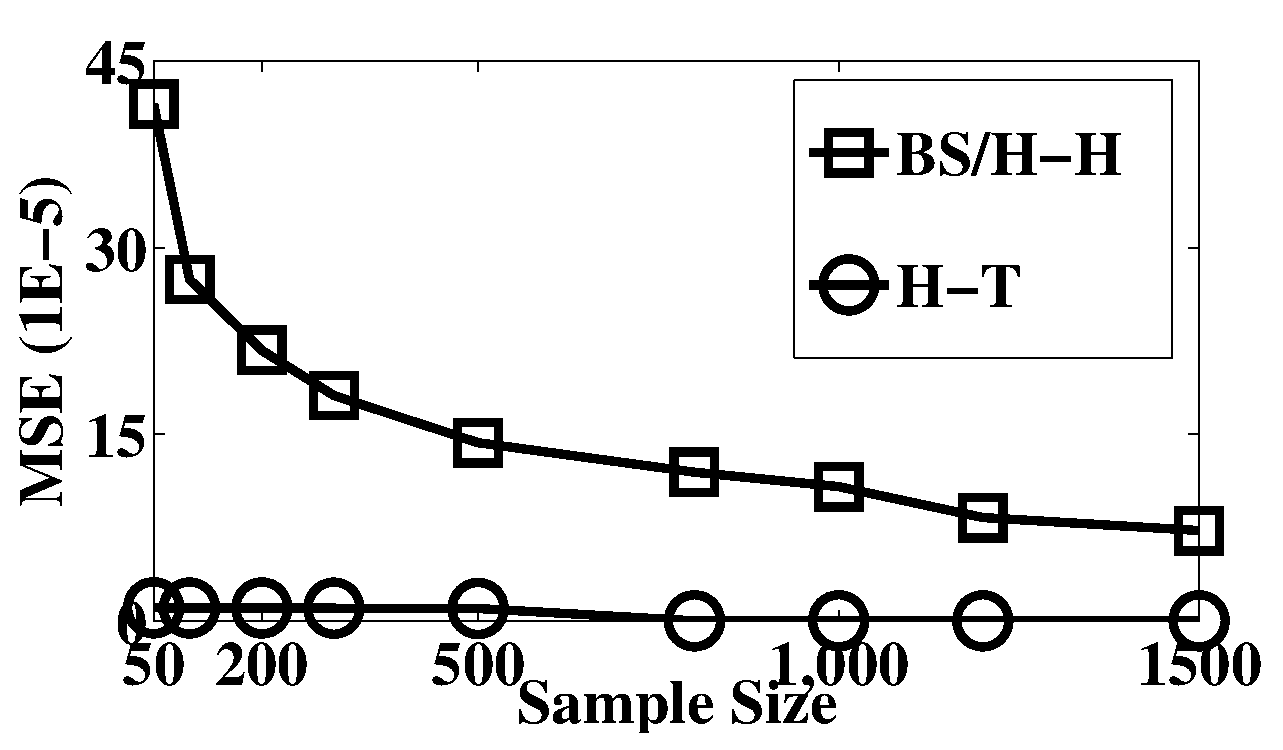
\includegraphics[width=0.32\textwidth]{fig-var-OL.eps}}
  \subfigure[\small{SF}]{
      \label{fig:mse:sf}
      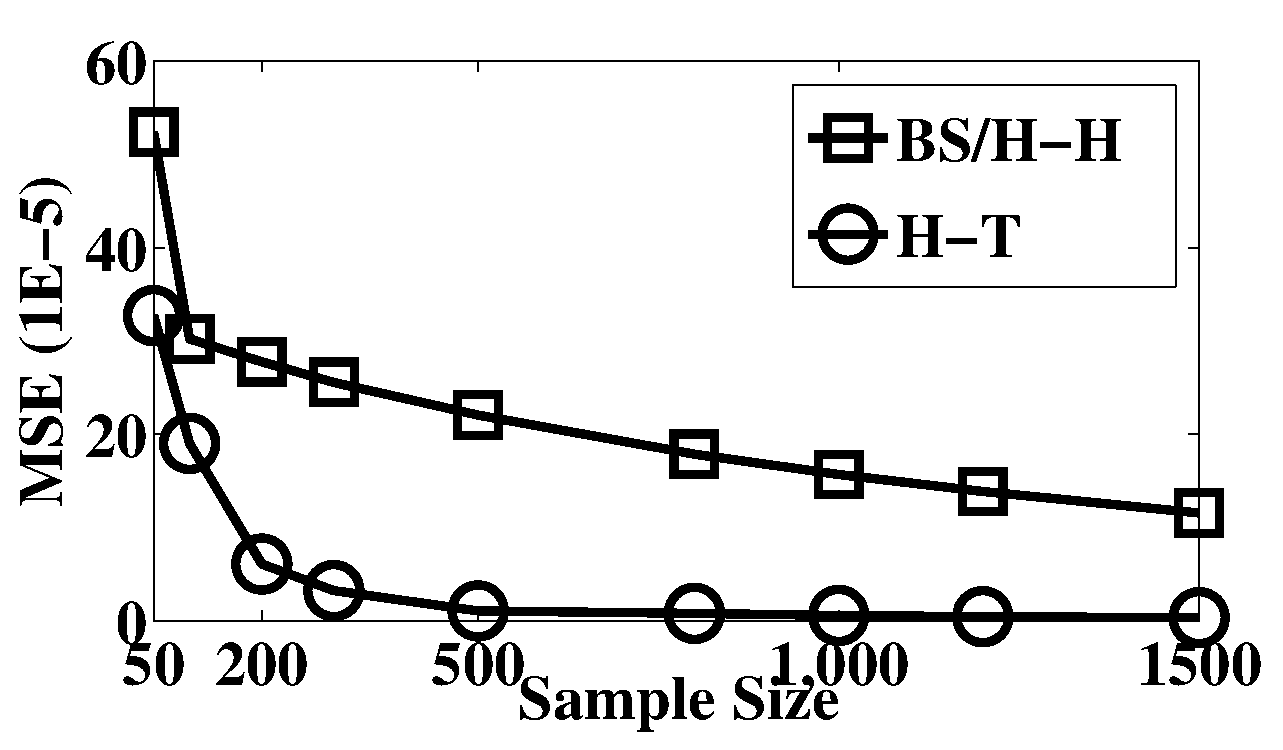
\includegraphics[width=0.32\textwidth]{fig-var-SF.eps}}
  \subfigure[\small{wiki-Vote}]{
      \label{fig:mse:wiki}
      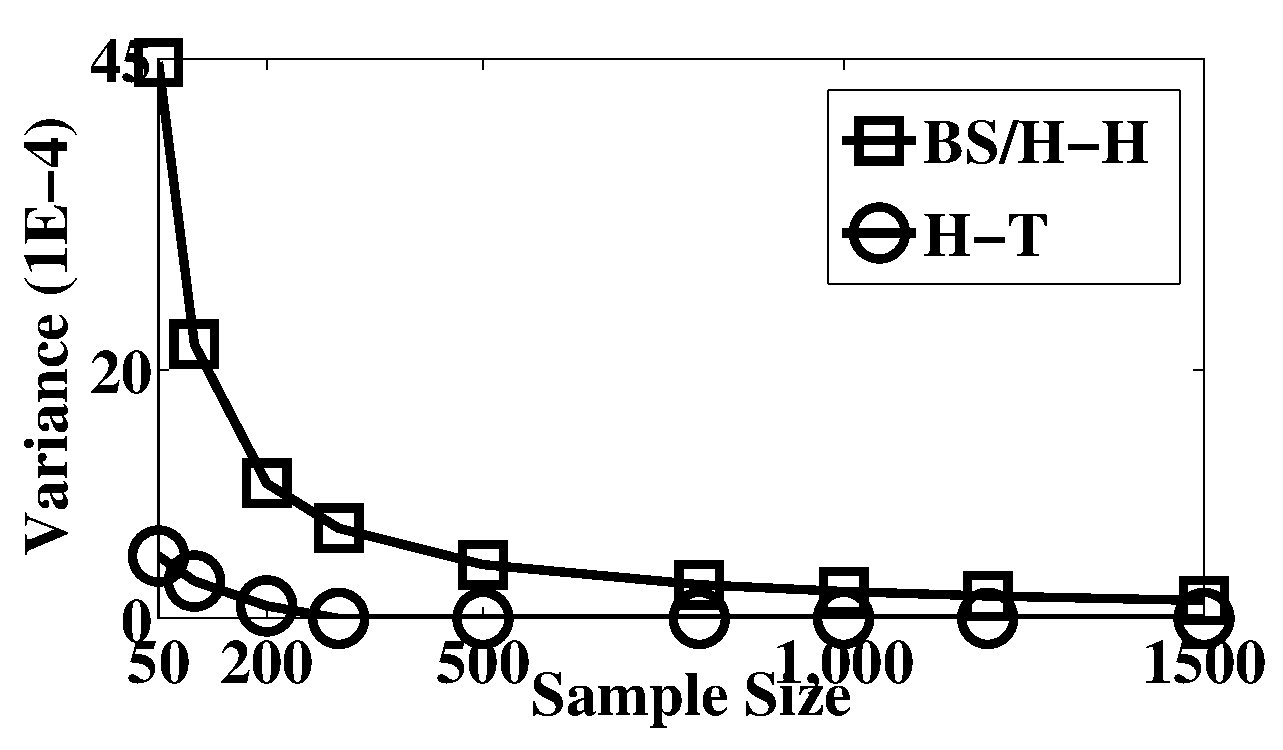
\includegraphics[width=0.32\textwidth]{fig-var-Wiki.eps}}
  %\subfigure[\small{soc-Epinions1}]{
%      \label{fig:mse:soc}
%      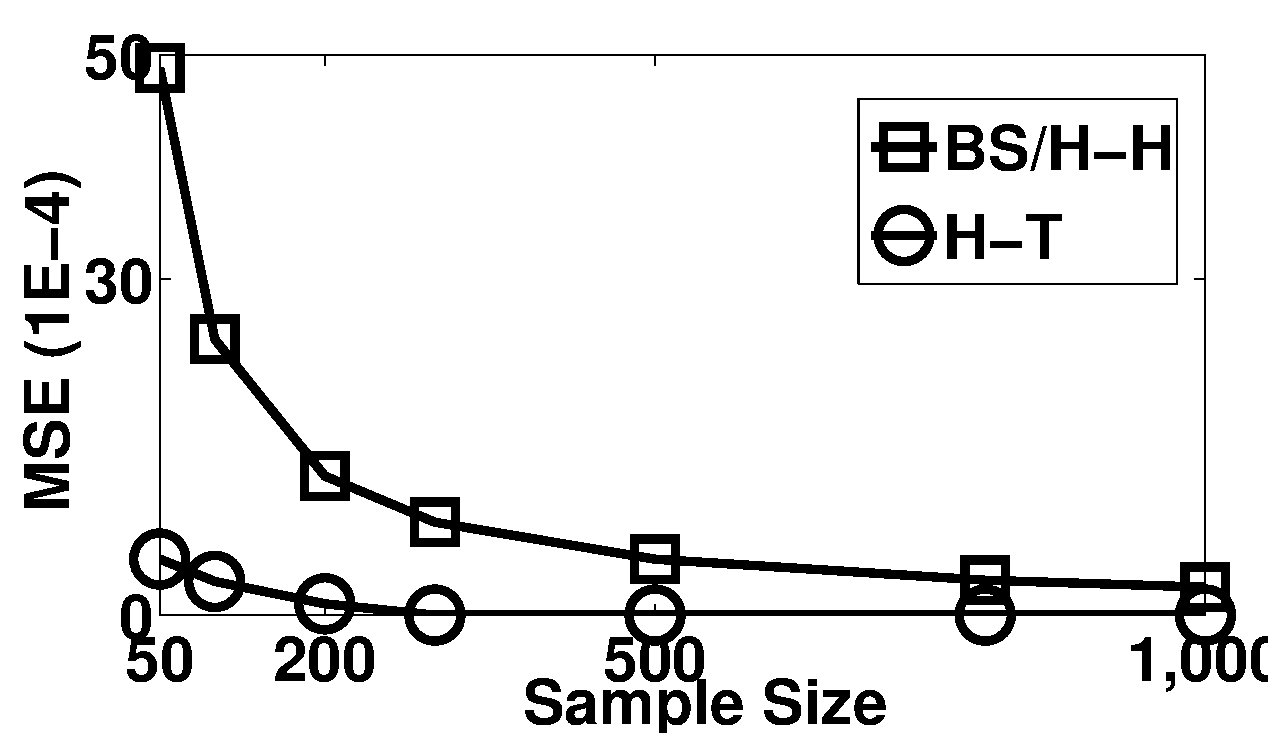
\includegraphics[width=0.4\textwidth]{fig-var-Soc.eps}}
\vspace{-0.3cm}
  \caption{Mean Square Error vs Sample Size}
  \label{fig:mse}
\vspace{-0.6cm}
\end{figure*}

From Fig.~\ref{fig:mse}, it can be seen that no matter how the size of datasets change, the variance of estimators decreases as sample size increases. Moreover, the variance of $\widehat{SPr_{H-T}}$ always keeps smaller than that of $\widehat{SPr_{H-H}}$. This result means the $\widehat{SPr_{H-T}}$ estimator is better than $\widehat{SPr_{H-T}}$, which verifies the discussion in Section~\ref{sec:sec:unequl-pro-samp}.

\begin{figure*}[htbp]
\vspace{-0.7cm}
  \centering
  \subfigure[\small{OL}]{
      \label{fig:error:ol}
      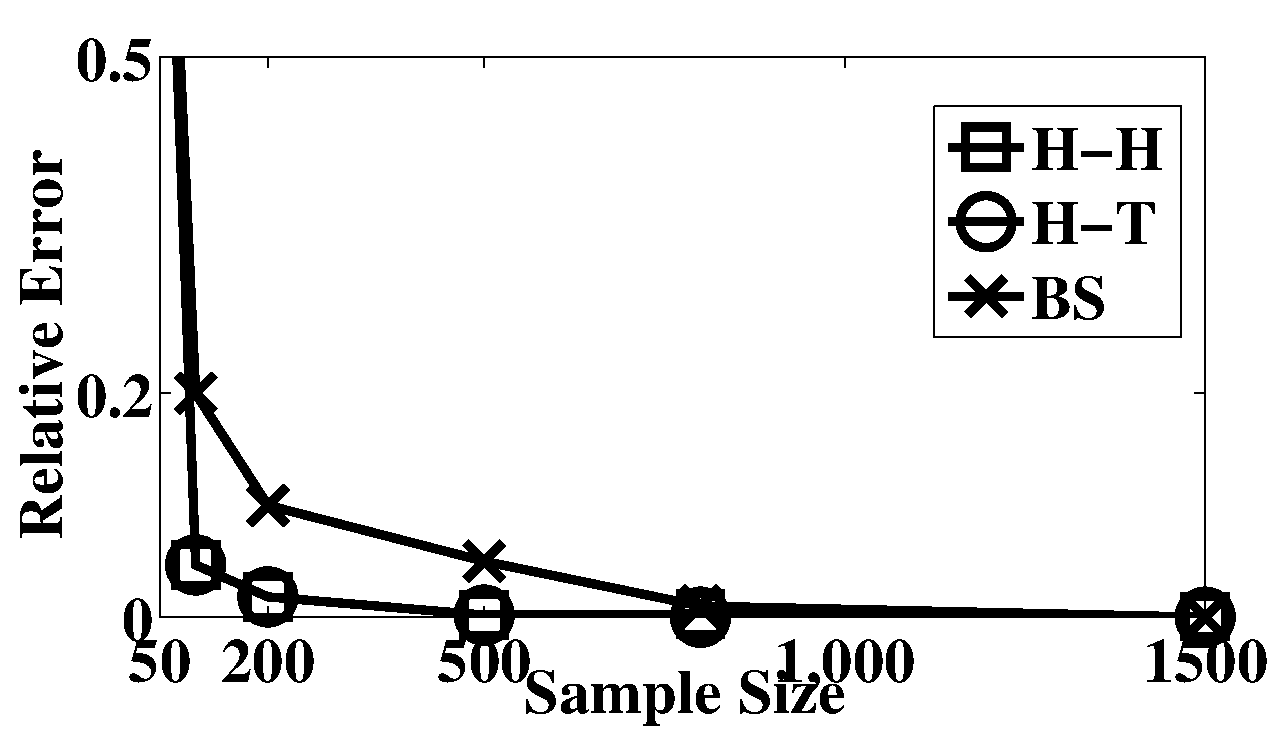
\includegraphics[width=0.32\textwidth]{fig-err-OL.eps}}
  \subfigure[\small{SF}]{
      \label{fig:error:sf}
      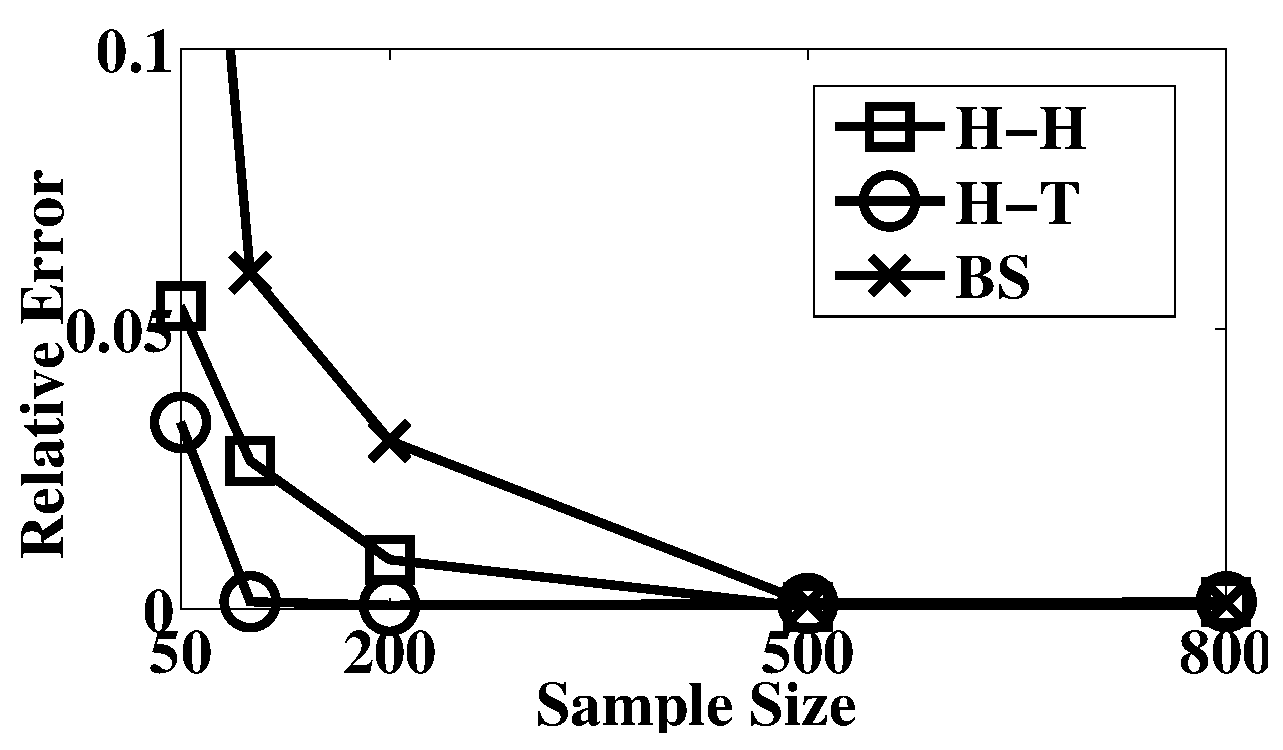
\includegraphics[width=0.32\textwidth]{fig-err-SF.eps}}
  \subfigure[\small{wiki-Vote}]{
      \label{fig:error:wiki}
      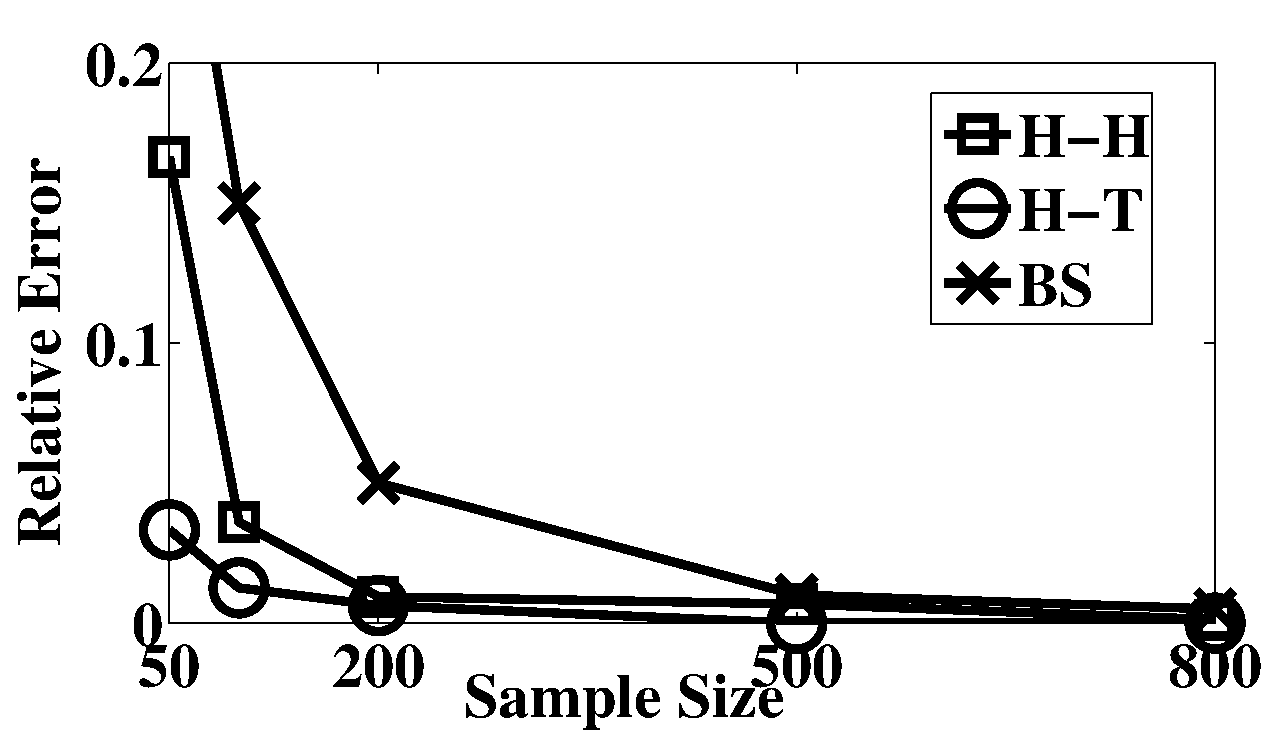
\includegraphics[width=0.32\textwidth]{fig-err-Wiki.eps}}
  %\subfigure[\small{soc-Epinions1}]{
%      \label{fig:error:soc}
%      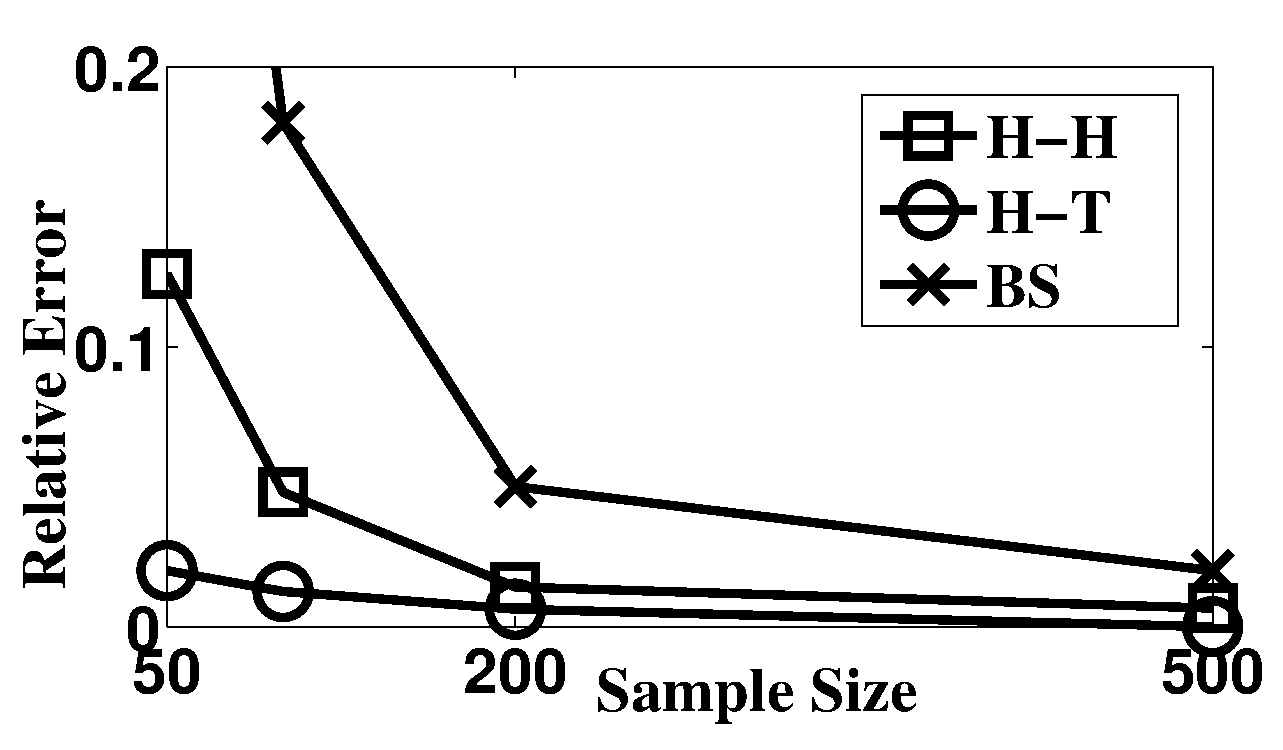
\includegraphics[width=0.4\textwidth]{fig-err-Soc.eps}}
\vspace{-0.3cm}
  \caption{Relative Error vs Sample Size}
  \label{fig:error}
\vspace{-0.6cm}
\end{figure*}

From Fig.~\ref{fig:error}, the relative error of \emph{BS} is always the largest, and \emph{H-T} of \emph{DS} is always the smallest. This means the stability and accuracy of $\widehat{SPr_{H-T}}$ is strongest. This result verifies our analysis in Section~\ref{sec:sec:DijSampling}. That is, we need fewer sampling times by applying \emph{DijSampling} Algorithm to get the same accuracy as baseline algorithm.

As we cannot get the distribution of unequal probability sampling, the error cannot be bounded. However, from Figure~\ref{fig:error}, in the 4 datasets used in our experiments, the error of both $\widehat{SPr_{H-T}}$ and $\widehat{SPr_{H-H}}$ is very low. Moreover, with the increase of sample times, the error fluctuates very gently. Thus, the estimators can approximate the exact answer well.


\vspace{-0.4cm}
\section{Related Works}
\label{sec:relate}
\vspace{-0.2cm}

The most popular shortest path algorithms over deterministic graphs are \emph{Dijkstra} \cite{bast2006transit} and $A^{*}$~\cite{fu2006heuristic}. These algorithms has a large time complexity. Thus, there are large number of works focusing on building indexes to speed up the algorithms. To accelerate the exact shortest path query, Cohen et al.~\cite{cohen2003reachability} proposed a 2-hop labeling method, and F.Wei~\cite{wei2010tedi} proposed a tree-width decomposition index. Moreover, authors in~\cite{gubichev2010fast} proposed a landmark encoding method to provide an approximate answer for shortest path query. In addition, there are also some shortest path algorithms over deterministic graphs designed typically for road networks such as~\cite{sankaranarayanan2009path}\cite{samet2008scalable}\cite{rice2010graph}\cite{jing1998hierarchical}, and \cite{wu2012shortest} is a good summary. In recent years, some shortest path algorithms are also designed to for large graph environment, such as \cite{jin2012highway}\cite{cheng2012efficient}\cite{gao2011relational}.

Essentially, the models of these algorithms above are all different from ours, so it is impossible to extend these algorithms directly.

Different queries are addressed in uncertain environment for a long time such as~\cite{tong2012mining} \cite{tong2012discovering}\cite{yuan2011efficient}\cite{yuan2013efficient}. Among them, shortest path query over uncertain graph is important. This query is first proposed by Loui~\cite{loui1983optimal}. Many works such as~\cite{yuan2010efficiently}\cite{zou2011top} considered an independent model, which is argued in detail in Section~\ref{sec:intro}. Moreover, Ming Hua et.al~\cite{hua2010probabilistic} built a simple correlated model. It modeled simple correlation in uncertain graphs between each two edges sharing the same vertex. But when there are more than two edges sharing the same vertex, it would be confusing.

In addition, ruoming Jin et.al~\cite{jin2011distance} applied \emph{Unequal Probability Sampling} method, which solved the uncertain reachability problem efficiently and effectively. However, their algorithms cannot be applied into our problem directly for three reasons. First, their model was independent uncertain graph model, and their algorithms cannot handle the correlated uncertain graph model. Secondly, their query was reachability, which is different from our shortest path query. As discussed in Section~\ref{sec:sec:pro-state}, our problem is harder than theirs. Thirdly, they applied their sampling algorithm in a \emph{divided and conquer} framework. If this framework is extended to our problem directly, we cannot find out the shortest path unless the last edge is sampled. Then, their algorithms would lose the advantages.

\vspace{-0.3cm}
%
\section{Conclusion}
%
\label{sec:conclu}
\vspace{-0.2cm}

In this paper, we first propose a new uncertain graph model, which considers the hidden correlation among edges sharing the same vertex. As calculating the \emph{shortest path probability} is a \#P-hard problem, we use sampling methods to approximately compute it. We propose a baseline algorithm and an improved algorithm. Our improved algorithm is more efficient than the baseline algorithm with more accurate answers when sampling the same times. Moreover, we preform comprehensive experiments to verify the efficiency and accuracy of our algorithms.


\vspace{-0.3cm}
\subsubsection*{Acknowledgments.} Yurong Cheng, Ye Yuan and Guoren Wang were supported by the NSFC
(Grant No.61025007, 61328202, 61202087, and 61100024), National Basic Research Program of China (973, Grant No.2011CB302200-G), National High Technology Research and Development 863 Program of China (Grant No.2012AA011004), and the Fundamental Research Funds for the Central Universities (Grant No. N110404011). Baiyou qiao was supported by the NSFC (Grant No.61073063).

\bibliographystyle{splncs03}
\bibliography{References}

\end{document}
